\documentclass[12pt,twoside]{report}
%%%%%%%%%%%%%%%%%%%%%%%%%%%%%%%%%%%%%%%%%%%%%%%%%%%%%%%%%%%%
% Unified definitions file.  Pulled together from various  %
% papers, the handbook, and so on.  Needs more work.       %
%%%%%%%%%%%%%%%%%%%%%%%%%%%%%%%%%%%%%%%%%%%%%%%%%%%%%%%%%%%%

\newenvironment{startarabicpagination}
{
	\setcounter{page}{1}
	\pagenumbering{arabic}
}
{}

\renewcommand{\epsilon}{\varepsilon}
\renewcommand{\rho}{\varrho}

\renewcommand{\ln}{\log}
\renewcommand{\hat}{\widehat}
\renewcommand{\tilde}{\widetilde}
\renewcommand{\leq}{\leqslant}
\renewcommand{\geq}{\geqslant}

\def\qed{\halmos}

\def\gm{\gamma}
\def\eps{\varepsilon}

\newcommand{\gr}{\mbox{$\nabla$}}

\newcommand{\graphCap}[4]{\begin{figure}  [hbt!]  \centering \includegraphics[scale = #2]{#1} \caption{#3}  \label{#4} \end{figure}} 

% e.g. \graphNoCap{birdDiag.jpg}{0.15}
\newcommand{\graphNoCap}[2]{\FloatBarrier \includegraphics[scale = #2]{#1} \FloatBarrier}

\newcommand{\dotsim}{\stackrel{\centerdot}{\sim}}

\def\acro#1#2{\vskip4pt\hbox to\textwidth{\normalsize
\hbox to5pc{#1\hfill}\vtop{\advance\hsize by
-5pc\raggedright\noindent#2}}}

\def\symbols{
\chapter*{List of Symbols}
\markboth{Symbols}{Symbols}
\addcontentsline{toc}{chapter}{\protect\numberline{\ }List of Symbols}}

\def\symbol#1#2{\vskip4pt\hbox to\textwidth{\normalsize
\hbox to5pc{#1\hfill}\vtop{\advance\hsize by
-5pc\raggedright\noindent#2}}}

\def\ack{\noindent {\bf Acknowledgements.\ }}

\newenvironment{proof}{ {\em \noindent Proof:} }{ }

%%%%%%%%%%%%%%%%%%%%%%%%%%%%%%%%%%%%%%%%%%%%%%%%%%%%%%%%%%%%
% Define new theorem environments                          %
%%%%%%%%%%%%%%%%%%%%%%%%%%%%%%%%%%%%%%%%%%%%%%%%%%%%%%%%%%%%

\newtheorem{example}{Example}[section]
\newtheorem{remark}{Remark}[section]
\newtheorem{algorithm}{Algorithm}[section]
\newtheorem{definition}{Definition}[section]
\newtheorem{lemma}{Lemma}[section]
\newtheorem{theorem}{Theorem}[section]
\newtheorem{proposition}{Proposition}[section]

\newtheorem{Def}{Definition}
\newtheorem{Thm}[Def]{Theorem}
\newtheorem{Lem}[Def]{Lemma}
\newtheorem{Cor}[Def]{Corollary}
\newtheorem{Prop}[Def]{Proposition}

\newtheorem{defin}{Definition}
\newtheorem{alg}{Algorithm}
\newtheorem{ass}{Assumption}

\newcounter{exctr}

%%%%%%%%%%%%%%%%%%%%%%%%%%%%%%%%%%%%%%%%%%%%%%%%%%%%%%%%%%%%
% Define abbreviated begin and end commands                %
%%%%%%%%%%%%%%%%%%%%%%%%%%%%%%%%%%%%%%%%%%%%%%%%%%%%%%%%%%%%

\newcommand{\balg}{\begin{algorithm}}
\newcommand{\ealg}{\end{algorithm}}

\newcommand{\ben}{\begin{enumerate}}
\newcommand{\een}{\end{enumerate}}

\newcommand{\beq}{\begin{equation}}
\newcommand{\eeq}{\end{equation}}

\newcommand{\eit}{\end{itemize}}
\newcommand{\bit}{\begin{itemize}}

\newcommand{\bex}{\begin{example}}
\newcommand{\eex}{\end{example}}

\newcommand{\blem}{\begin{lem}}
\newcommand{\elem}{\end{lem}}

\newcommand{\bthm}{\begin{theorem}}
\newcommand{\ethm}{\end{theorem}}

\newcommand{\bdsc}{\begin{description}}
\newcommand{\edsc}{\end{description}}


\newcommand{\brem}{\begin{remark}}
\newcommand{\erem}{\end{remark}}

\newcommand{\bprop}{\begin{proposition}}
\newcommand{\eprop}{\end{proposition}}




%%%%%%%%%%%%%%%%%%%%%%%%%%%%%%%%%%%%%%%%%%%%%%%%%%%%%%%%%%%%
%                                                          %
%%%%%%%%%%%%%%%%%%%%%%%%%%%%%%%%%%%%%%%%%%%%%%%%%%%%%%%%%%%%

\newcommand{\st}{\: : \:} % such that

\newcommand{\ceil}[1]{\left\lceil #1 \right\rceil}
\newcommand{\floor}[1]{\left\lfloor #1 \right\rfloor}

\newcommand{\Shan}{\EuScript{H}}
\newcommand{\KL}{\EuScript{D}}
\newcommand{\El}{{\EuScript{E}}}
\newcommand{\MI}{\EuScript{M}} % mutual information
\newcommand{\Lh}{\EuScript{L}} % likelihood
\newcommand{\LR}{\EuScript{W}} % likelihood ratio
\newcommand{\Fish}{\EuScript{I}}
\newcommand{\Sc}{\EuScript{S}} % score function
\newcommand{\bigO}{\EuScript{O}}
\newcommand{\lito}{$o$}

\newcommand{\pf}{L} % performance function

%\newcommand{\D}{\mathfrak{D}}

\newcommand{\bincof}[2]{{{#1} \choose {#2}}}



%%%%%%%%%%%%%%%%%%%%%%%%%%%%%%%%%%%%%%%%%%%%%%%%%%%%%%%%%%%%
% Define \b? as \mathbf{?}                                 %
% Exception: \bff for \mathbf{f}                           %
%%%%%%%%%%%%%%%%%%%%%%%%%%%%%%%%%%%%%%%%%%%%%%%%%%%%%%%%%%%%

\newcommand{\ba}{\mathbf{a}}
\newcommand{\bA}{\mathbf{A}}
\newcommand{\bb}{\mathbf{b}}
\newcommand{\bB}{\mathbf{B}}
\newcommand{\bc}{\mathbf{c}}
\newcommand{\bC}{\mathbf{C}}
\newcommand{\bd}{\mathbf{d}}
\newcommand{\bD}{\mathbf{D}}
\newcommand{\be}{\mathbf{e}}
\newcommand{\bE}{\mathbf{E}}
\newcommand{\bff}{\mathbf{f}}
\newcommand{\bF}{\mathbf{F}}
\newcommand{\bg}{\mathbf{g}}
\newcommand{\bG}{\mathbf{G}}
\newcommand{\bh}{\mathbf{h}}
\newcommand{\bH}{\mathbf{H}}
\newcommand{\bi}{\mathbf{i}}
\newcommand{\bI}{\mathbf{I}}
\newcommand{\bj}{\mathbf{j}}
\newcommand{\bJ}{\mathbf{J}}
\newcommand{\bk}{\mathbf{k}}
\newcommand{\bK}{\mathbf{K}}
\newcommand{\bl}{\mathbf{l}}
\newcommand{\bL}{\mathbf{L}}
\newcommand{\bm}{\mathbf{m}}
\newcommand{\bM}{\mathbf{M}}
\newcommand{\bn}{\mathbf{n}}
\newcommand{\bN}{\mathbf{N}}
\newcommand{\bo}{\mathbf{o}}
\newcommand{\bO}{\mathbf{O}}
\newcommand{\bp}{\mathbf{p}}
\newcommand{\bP}{\mathbf{P}}
\newcommand{\bq}{\mathbf{q}}
\newcommand{\bQ}{\mathbf{Q}}
\newcommand{\br}{\mathbf{r}}
\newcommand{\bR}{\mathbf{R}}
\newcommand{\bs}{\mathbf{s}}
\newcommand{\bS}{\mathbf{S}}
\newcommand{\bt}{\mathbf{t}}
\newcommand{\bT}{\mathbf{T}}
\newcommand{\bu}{\mathbf{u}}
\newcommand{\bU}{\mathbf{U}}
\newcommand{\bv}{\mathbf{v}}
\newcommand{\bV}{\mathbf{V}}
\newcommand{\bw}{\mathbf{w}}
\newcommand{\bW}{\mathbf{W}}
\newcommand{\bx}{\mathbf{x}}
\newcommand{\bX}{\mathbf{X}}
\newcommand{\by}{\mathbf{y}}
\newcommand{\bY}{\mathbf{Y}}
\newcommand{\bz}{\mathbf{z}}
\newcommand{\bZ}{\mathbf{Z}}


%%%%%%%%%%%%%%%%%%%%%%%%%%%%%%%%%%%%%%%%%%%%%%%%%%%%%%%%%%%%
% Define \vect{}, and \b* for \vect{*} with Greek letters  %
% Exception: \bfeta for \vect{\eta}                        %
%%%%%%%%%%%%%%%%%%%%%%%%%%%%%%%%%%%%%%%%%%%%%%%%%%%%%%%%%%%%

\newcommand{\vect}[1]{\boldsymbol #1}

\newcommand{\balpha}{\vect{\alpha}}
\newcommand{\bAlpha}{\vect{\Alpha}}
\newcommand{\bbeta}{\vect{\beta}}
\newcommand{\bBeta}{\vect{\Beta}}
\newcommand{\bgamma}{\vect{\gamma}}
\newcommand{\bGamma}{\vect{\Gamma}}
\newcommand{\bdelta}{\vect{\delta}}
\newcommand{\bDelta}{\vect{\Delta}}
\newcommand{\bepsilon}{\vect{\epsilon}}
\newcommand{\bEpsilon}{\vect{\Epsilon}}
\newcommand{\bzeta}{\vect{\zeta}}
\newcommand{\bZeta}{\vect{\Zeta}}
\newcommand{\bfeta}{\vect{\eta}}
\newcommand{\bEta}{\vect{\Eta}}
\newcommand{\btheta}{\vect{\theta}}
\newcommand{\bTheta}{\vect{\Theta}}
\newcommand{\biota}{\vect{\iota}}
\newcommand{\bIota}{\vect{\Iota}}
\newcommand{\bkappa}{\vect{\kappa}}
\newcommand{\bKappa}{\vect{\Kappa}}
\newcommand{\blambda}{\vect{\lambda}}
\newcommand{\bLambda}{\vect{\Lambda}}
\newcommand{\bmu}{\vect{\mu}}
\newcommand{\bMu}{\vect{\Mu}}
\newcommand{\bnu}{\vect{\nu}}
\newcommand{\bNu}{\vect{\Nu}}
\newcommand{\bxi}{\vect{\xi}}
\newcommand{\bXi}{\vect{\Xi}}
\newcommand{\bomricon}{\vect{\omricon}}
\newcommand{\bOmricon}{\vect{\Omricon}}
\newcommand{\bpi}{\vect{\pi}}
\newcommand{\bPi}{\vect{\Pi}}
\newcommand{\brho}{\vect{\rho}}
\newcommand{\bRho}{\vect{\Rho}}
\newcommand{\bsigma}{\vect{\sigma}}
\newcommand{\bSigma}{\vect{\Sigma}}
\newcommand{\btau}{\vect{\tau}}
\newcommand{\bTau}{\vect{\Tau}}
\newcommand{\bupsilon}{\vect{\upsilon}}
\newcommand{\bUpsilon}{\vect{\Upsilon}}
\newcommand{\bphi}{\vect{\phi}}
\newcommand{\bPhi}{\vect{\Phi}}
\newcommand{\bchi}{\vect{\chi}}
\newcommand{\bChi}{\vect{\Chi}}
\newcommand{\bpsi}{\vect{\psi}}
\newcommand{\bPsi}{\vect{\Psi}}
\newcommand{\bomega}{\vect{\omega}}
\newcommand{\bOmega}{\vect{\Omega}}



%%%%%%%%%%%%%%%%%%%%%%%%%%%%%%%%%%%%%%%%%%%%%%%%%%%%%%%%%%%%
% Define \v? for \mathcal{?}                               %
%%%%%%%%%%%%%%%%%%%%%%%%%%%%%%%%%%%%%%%%%%%%%%%%%%%%%%%%%%%%

\newcommand{\cA}{\mathcal{A}}
\newcommand{\cB}{\mathcal{B}}
\newcommand{\cC}{\mathcal{C}}
\newcommand{\cD}{\mathcal{D}}
\newcommand{\cE}{\mathcal{E}}
\newcommand{\cF}{\mathcal{F}}
\newcommand{\cG}{\mathcal{G}}
\newcommand{\cH}{\mathcal{H}}
\newcommand{\cI}{\mathcal{I}}
\newcommand{\cJ}{\mathcal{J}}
\newcommand{\cK}{\mathcal{K}}
\newcommand{\cL}{\mathcal{L}}
\newcommand{\cM}{\mathcal{M}}
\newcommand{\cN}{\mathcal{N}}
\newcommand{\cO}{\mathcal{O}}
\newcommand{\cP}{\mathcal{P}}
\newcommand{\cQ}{\mathcal{Q}}
\newcommand{\cR}{\mathcal{R}}
\newcommand{\cS}{\mathcal{S}}
\newcommand{\cT}{\mathcal{T}}
\newcommand{\cU}{\mathcal{U}}
\newcommand{\cV}{\mathcal{V}}
\newcommand{\cW}{\mathcal{W}}
\newcommand{\cX}{\mathcal{X}}
\newcommand{\cY}{\mathcal{Y}}
\newcommand{\cZ}{\mathcal{Z}}



%%%%%%%%%%%%%%%%%%%%%%%%%%%%%%%%%%%%%%%%%%%%%%%%%%%%%%%%%%%%
% Define \sc? for \mathscr{?}                              %
%%%%%%%%%%%%%%%%%%%%%%%%%%%%%%%%%%%%%%%%%%%%%%%%%%%%%%%%%%%%

\newcommand{\scA}{\mathscr{A}}
\newcommand{\scB}{\mathscr{B}}
\newcommand{\scC}{\mathscr{C}}
\newcommand{\scD}{\mathscr{D}}
\newcommand{\scE}{\mathscr{E}}
\newcommand{\scF}{\mathscr{F}}
\newcommand{\scG}{\mathscr{G}}
\newcommand{\scH}{\mathscr{H}}
\newcommand{\scI}{\mathscr{I}}
\newcommand{\scJ}{\mathscr{J}}
\newcommand{\scK}{\mathscr{K}}
\newcommand{\scL}{\mathscr{L}}
\newcommand{\scM}{\mathscr{M}}
\newcommand{\scN}{\mathscr{N}}
\newcommand{\scO}{\mathscr{O}}
\newcommand{\scP}{\mathscr{P}}
\newcommand{\scQ}{\mathscr{Q}}
\newcommand{\scR}{\mathscr{R}}
\newcommand{\scS}{\mathscr{S}}
\newcommand{\scT}{\mathscr{T}}
\newcommand{\scU}{\mathscr{U}}
\newcommand{\scV}{\mathscr{V}}
\newcommand{\scW}{\mathscr{W}}
\newcommand{\scX}{\mathscr{X}}
\newcommand{\scY}{\mathscr{Y}}
\newcommand{\scZ}{\mathscr{Z}}


%%%%%%%%%%%%%%%%%%%%%%%%%%%%%%%%%%%%%%%%%%%%%%%%%%%%%%%%%%%%
% Define \d? for \text{d}? and \db? for \text{d}\b?        %
% Runs from r to z and \br to \bz                          %
%%%%%%%%%%%%%%%%%%%%%%%%%%%%%%%%%%%%%%%%%%%%%%%%%%%%%%%%%%%%

\newcommand{\dr}{{\text{d}r}}
\newcommand{\ds}{{\text{d}s}}
\newcommand{\dt}{{\text{d}t}}
\newcommand{\du}{{\text{d}u}}
\newcommand{\dv}{{\text{d}v}}
\newcommand{\dw}{{\text{d}w}}
\newcommand{\dx}{{\text{d}x}}
\newcommand{\dy}{{\text{d}y}}
\newcommand{\dz}{{\text{d}z}}

\newcommand{\dF}{{\text{d}F}}
\newcommand{\dG}{{\text{d}G}}

\newcommand{\dbr}{{\text{d}\br}}
\newcommand{\dbs}{{\text{d}\bs}}
\newcommand{\dbt}{{\text{d}\bt}}
\newcommand{\dbu}{{\text{d}\bu}}
\newcommand{\dbv}{{\text{d}\bv}}
\newcommand{\dbw}{{\text{d}\bw}}
\newcommand{\dbx}{{\text{d}\bx}}
\newcommand{\dby}{{\text{d}\by}}
\newcommand{\dbz}{{\text{d}\bz}}






\newcommand{\rfp}[1]{(\ref{#1})}
\newcommand{\refp}[1]{(\ref{#1})}
\newcommand{\refs}[1]{(\ref{#1})}
\newcommand{\refds}[2]{({#1}.\ref{#2})}



\newcommand{\halmos}{\vspace{3mm} \hfill \mbox{$\Box$}}



\newcommand{\widetildeS}{\widetilde{S}}
\newcommand{\vvv}[1]{\mbox{\boldmath$#1$}}

%%%%%%%%%%%%%%%%%%%%%%%%%%%%%%%%%%%%%%%%%%%%%%%%%%%%%%%%%%%%
% Define common \text{} typeset elements for mathmode      %
%%%%%%%%%%%%%%%%%%%%%%%%%%%%%%%%%%%%%%%%%%%%%%%%%%%%%%%%%%%%

\newcommand{\Var}{\text{Var}}
\newcommand{\var}{\Var}
\newcommand{\Std}{\text{Std}}
\newcommand{\std}{\Std}
\newcommand{\Cov}{\text{Cov}}
\newcommand{\cov}{\Cov}
\newcommand{\Supp}{\text{Supp}}
\newcommand{\supp}{\Supp}
\newcommand{\SCV}{\text{SCV}}
\newcommand{\RE}{\text{RE}}
%\renewcommand{\skew}{\text{Skew}}

\newcommand{\I}{\text{I}}

\newcommand{\indicator}[1]{\mbox{{\rm I}}_{\{#1\}}}


%%%%%%%%%%%%%%%%%%%%%%%%%%%%%%%%%%%%%%%%%%%%%%%%%%%%%%%%%%%%
% Define new \mathops                                      %
%%%%%%%%%%%%%%%%%%%%%%%%%%%%%%%%%%%%%%%%%%%%%%%%%%%%%%%%%%%%

\newcommand{\argmax}{\mathop{\rm argmax}}
\newcommand{\argmin}{\mathop{\rm argmin}}
\newcommand{\elite}{\mathop{\rm elite}}
\newcommand{\diag}{\mathop{\rm diag}}
\newcommand{\nondiag}{\mathop{\rm nondiag}}
\newcommand{\fin}{\mathop{\rm fin}}
\newcommand{\start}{\mathop{\rm start}}
\newcommand{\tot}{\mathop{\rm tot}}
\newcommand{\difr}{\mathop{\rm difr}}

\newcommand{\iid}{\text{iid }}

\newcommand{\sgn}{\text{sgn}}

\newcommand{\tr}{\text{tr}}

%\newcommand{\cas}{{\stackrel{\text{a.s.}}{\longrightarrow}\: }}

\newcommand{\Ito}{It\^{o}}

\newcommand{\obs}{\mathop{\rm obs}}
\newcommand{\mis}{\mathop{\rm mis}}
\newcommand{\Conv}{\mathop{\mathbf{Conv}}}





%%%%%%%%%%%%%%%%%%%%%%%%%%%%%%%%%%%%%%%%%%%%%%%%%%%%%%%%%%%%
% Define statistical distributions                         %
%%%%%%%%%%%%%%%%%%%%%%%%%%%%%%%%%%%%%%%%%%%%%%%%%%%%%%%%%%%%

\newcommand{\Ber}{{\sf Ber}}
\newcommand{\ber}{\Ber}
\newcommand{\Bin}{{\sf Bin}}
\newcommand{\bin}{\Bin}

\newcommand{\Dir}{{\sf Dir}}
\newcommand{\Erl}{{\sf Erl}}

\newcommand{\Geo}{{\sf Geom}}
\newcommand{\geo}{\Geo}

\newcommand{\G}{\Geo}

\newcommand{\Poi}{{\sf Poi}}
\newcommand{\poi}{\Poi}

\newcommand{\Bet}{{\sf Beta}}
\newcommand{\bet}{\Bet}
\newcommand{\Cauchy}{{\sf Cauchy}}
\newcommand{\cauchy}{\Cauchy}
\newcommand{\Ex}{{\sf Exp}}
\newcommand{\ex}{\Ex}
\newcommand{\Gam}{{\sf Gam}}
\newcommand{\gam}{\Gam}
\newcommand{\Nor}{{\sf N}}
\newcommand{\nor}{\Nor}
\newcommand{\U}{{\sf U}}
%\newcommand{\u}{\U}
\newcommand{\Weib}{{\sf Weib}}
\newcommand{\weib}{\Weib}

%\newcommand{\NE}{\sf NE}
%\newcommand{\Hyp}{\sf Hyp}
%\newcommand{\pareto}{\sf Pareto} % pareto
%\newcommand{\DU}{\sf DU}
%\newcommand{\SE}{\sf SExp} % shifted exponential
%\newcommand{\DE}{\sf DExp} % double exponential
%\newcommand{\nbin}{\sf NBin}

%\newcommand{\negbin}{{\sf NegBin}}
%\newcommand{\mnom}{{\sf Mnom}}
%\newcommand{\NE}{{\sf NE}}
%\newcommand{\Hyp}{{\sf Hyp}}
%\newcommand{\pareto}{{\sf Pareto}} % pareto
%\newcommand{\NegHyp}{{\sf NegHyp}}
%\newcommand{\DiscPhase}{{\sf PH}}
%\newcommand{\ContPhase}{{\sf PH}}
%\newcommand{\DExp}{{\sf DExp}}
%\newcommand{\F}{{\sf F}}
%\newcommand{\EVI}{{\sf ExValueI}}
%\newcommand{\EVII}{{\sf ExValueII}}
%\newcommand{\EVIII}{{\sf ExValueIII}}
%\newcommand{\IGauss}{{\sf InvGauss}}
%\newcommand{\logistic}{{\sf Logistic}}
\newcommand{\LogN}{{\sf LogN}}
%\newcommand{\Pareto}{{\sf Pareto}}
%\newcommand{\Ray}{{\sf Rayleigh}}
%\newcommand{\Stable}{{\sf Stable}}
%\newcommand{\student}{{\sf t}}
%\newcommand{\vonMises}{{\sf vonMises}}
%\newcommand{\Dirichlet}{{\sf Dirichlet}}
%\newcommand{\DU}{{\sf DU}}
%\newcommand{\SE}{{\sf SExp}} % shifted exponential
%\newcommand{\DE}{{\sf DExp}} % double exponential
%\newcommand{\nbin}{{\sf NBin}}


%%%%%%%%%%%%%%%%%%%%%%%%%%%%%%%%%%%%%%%%%%%%%%%%%%%%%%%%%%%%
% Define special symbols, such as expectation operator,    %
% probability measure, the reals, &c.                      %
%%%%%%%%%%%%%%%%%%%%%%%%%%%%%%%%%%%%%%%%%%%%%%%%%%%%%%%%%%%%

\newcommand{\Em}{\mathbb E}
\newcommand{\X}{\mathbb E}
\newcommand{\Pm}{\mathbb P}
\newcommand{\Qm}{\mathbb Q}
\newcommand{\Um}{\mathbb U}

\newcommand{\Prob}{\Pm}

\newcommand{\convdistr}{\stackrel{\cal D}{\rightarrow}}

\newcommand{\IZ}[1]{I_{\{\M(Z)>#1\}}}

\newcommand{\R}{\mathbb R}
\newcommand{\B}{\cal B}
\newcommand{\N}{\mathbb N}
\newcommand{\Z}{\mathbb Z}
\newcommand{\Q}{\mathbb Q}
\newcommand{\C}{\mathbb C}

\newcommand{\Rbar}{\overline{\R}}


\newcommand{\gvn}{\,|\,}
\newcommand{\biggvn}{\,\right|\left.\,}
\newcommand{\e}{\mbox{e}}
\renewcommand{\i}{\mbox{i}}



%%%%%%%%%%%%%%%%%%%%%%%%%%%%%%%%%%%%%%%%%%%%%%%%%%%%%%%%%%%%
%                                                          %
%%%%%%%%%%%%%%%%%%%%%%%%%%%%%%%%%%%%%%%%%%%%%%%%%%%%%%%%%%%%

\newcommand{\fb}{\rule[-2pt]{4pt}{8pt}}
\newcommand{\HS}[1][1.]{\hspace{\stretch{#1}}}

\newcommand{\chg}{\marginpar{*}}

\newcommand{\margref}[1]{\marginpar{{\quad {\large \ding{43}}
\pageref{#1}}}}

\newenvironment{codebox}{ \small \bigskip \breakbox
\verbatim \leftskip=8pt \vskip-10pt
}{ \endverbatim \vskip-8pt \endbreakbox \bigskip}

\newcommand{\term}[2]{\vskip2pt{\bf #1}\hskip1em #2}

\newcommand{\intrusion}[1]{\begin{list}{}%
{\leftmargin\parindent\rightmargin0pt\listparindent0pt\parsep1ex%
\labelwidth0pt\labelsep0pt}\item[]\small\sf$\maltese$~#1 \end{list}}



%%%%%%%%

%\newcommand{\xo}{\ensuremath{x_{\mathrm{eq}}}}
\newcommand{\xo}{\ensuremath{\bx_{\mathrm{eq}}}}
%\newcommand{\xs}{\ensuremath{x_{\mathrm{st}}}}
\newcommand{\xs}{\ensuremath{\bx_{\mathrm{st}}}}

\newcommand\myprime{\ensuremath{\,\prime}}

\def\OU{Ornstein-Uhlenbeck}


\newcommand{\Uppsi}{\Psi}
\newcommand{\mbf}[1]{\mathbf #1}

\newcommand{\littleo}{o}

\newcommand{\D}[2]{\mathcal{D}(#1\to#2)}
\newcommand{\Dtwo}[3]{\mathcal{D}_{#1}(#2\to#3)}
\newcommand{\Dphi}[2]{\mathcal{D}_\phi(#1\to#2)}

\newcommand{\tick}{\ding{51}}

\newcommand{\cross}{\ding{55}}

\newcommand{\LDlim}{\lim_{n\to\infty}\frac 1n \log}
\newcommand{\LDlimsup}{\limsup_{n\to\infty}\frac 1n \log}
\newcommand{\LDliminf}{\liminf_{n\to\infty}\frac 1n \log}
\newcommand{\isindist}{\stackrel{\rm d}{=}}
\newcommand{\defis}{\stackrel{\rm def}{=}}

\newcommand{\LDlimg}{\lim_{\gamma\to\infty}\frac 1\gamma \log}
\newcommand{\LDlimsupg}{\limsup_{\gamma\to\infty}\frac 1\gamma \log}
\newcommand{\LDliminfg}{\liminf_{\gamma\to\infty}\frac 1\gamma \log}


\newcommand{\Nset}{\N}
\newcommand{\Rset}{\R}

\newcommand{\di}{{\rm d}}

\let\origdoublepage\cleardoublepage
\newcommand{\clearemptydoublepage}{%
 \clearpage
{\pagestyle{empty}\origdoublepage}%
}

\let\cleardoublepage\clearemptydoublepage


\newcommand{\cas}{{\stackrel{\mathrm{a.s.}}{\longrightarrow}\: }}

\newcommand{\ra}{\rightarrow}
\newcommand{\Ra}{\Rightarrow}
\newcommand{\lra}{\leftrightarrow}
\newcommand{\da}{\downarrow}
\newcommand{\Da}{\Downarrow}


\renewcommand{\v}[1]{\boldsymbol{#1}}
\newcommand{\m}[1]{\mathbf{#1}}
\renewcommand{\c}[1]{\mathcal{#1}}
\newcommand{\s}[1]{\mathscr{#1}}
\newcommand{\iidsim}{\stackrel{\mathrm{iid}}{\sim}}
\newcommand{\simiid}{\iidsim}
\newcommand{\simiidt}{{\:{\sim}_{\mathrm{iid}}\:}}
%\newcommand{\diag}{\mathrm{diag}}
\newcommand{\cp}{\stackrel{\bb {P}}{\longrightarrow}}
\newcommand{\cd}{\stackrel{\mathrm{d}}{\longrightarrow}}

\newcommand{\T}{\top} 

\newcommand{\cmark}{\ding{51}}%
\newcommand{\xmark}{\ding{55}}%
\usepackage[utf8]{inputenc}
\usepackage{graphicx}
\graphicspath{ {images/} }
\usepackage{caption}
\usepackage{subcaption}
\usepackage[a4paper,width=150mm,top=25mm,bottom=25mm,bindingoffset=6mm]{geometry}
%\usepackage{fullpage}
%\usepackage[top=2cm, bottom=4.5cm, left=2.5cm, right=2.5cm]{geometry}
\let\proof\relax
\usepackage{amsmath,amsfonts,amssymb,amscd}
\let\endproof\relax
\usepackage{lastpage}
\usepackage{enumerate}
\usepackage{fancyhdr}
\usepackage{mathrsfs}
\usepackage{xcolor}
\usepackage{verbatim}
\usepackage{fancyvrb}
\usepackage{amsthm}
\usepackage{listings}
\usepackage{hyperref}
\usepackage{bbm}
\usepackage{dirtytalk}
\usepackage{fancyhdr}
\usepackage[section]{placeins}
\pagestyle{fancy}
\fancyhead{}
\fancyhead[RO,LE]{Games on Random Graphs}
\fancyfoot{}
\fancyfoot[LE,RO]{\thepage}
\fancyfoot[LO,CE]{Chapter \thechapter}
\fancyfoot[CO,RE]{Daniel Gray}
\renewcommand{\headrulewidth}{0.4pt}
\renewcommand{\footrulewidth}{0.4pt}
\setlength{\parindent}{0pt}
\usepackage[backend=biber,style=ieee,sorting=ynt, isbn=false, url = false]{biblatex} %best style is ieee, sorting = ynt
\usepackage{changepage}
\newenvironment{ltab}{\begin{adjustwidth}{2cm}{}}{\end{adjustwidth}}
\addbibresource{final3.bib} 

%workklow for bib is: store them in endnote, then export as .bib. Open in jabref and do unabbreviate journals, then export out as bib and import here

\title{Games on Random Graphs}
\author{Daniel Gray}
\date{\today}

\begin{document}

\begin{titlepage}
    \begin{center}
        \vspace*{1cm}
        
        \Huge
        \textbf{Evolutionary Game Theory on Random Graphs}
        
        \vspace{0.5cm}
        \LARGE
        %Thesis Subtitle
        
        \vspace{1.5cm}
        
        \textbf{Daniel Gray}
        
        \LARGE
        Supervised by Dr. Thomas Taimre
        
        \vspace{1.5cm}
        
        \vfill
        
        A thesis presented for \\ Mathematics Honours
        
        \vspace{0.8cm}
        

        
        \Large
        School of Mathematics and Physics\\
        University of Queensland\\
        Australia\\
        \today
        
    \end{center}
\end{titlepage}

%\thispagestyle{plain}
\begin{center}
    \Large
    \textbf{Thesis Title}
    
    \vspace{0.4cm}
    \large
    Thesis Subtitle
    
    \vspace{0.4cm}
    \textbf{Author Name}
    
    \vspace{0.9cm}
    \textbf{Abstract}
\end{center}
Lorem ipsum dolor sit amet, consectetur adipisicing elit, sed do eiusmod tempor incididunt ut labore et dolore magna aliqua. Ut enim ad minim veniam, quis nostrud exercitation ullamco laboris nisi ut aliquip ex ea commodo consequat. Duis aute irure dolor in reprehenderit in voluptate velit esse cillum dolore eu fugiat nulla pariatur. Excepteur sint occaecat cupidatat non proident, sunt in culpa qui officia deserunt mollit anim id est laborum.

Lorem ipsum dolor sit amet, consectetur adipisicing elit, sed do eiusmod tempor incididunt ut labore et dolore magna aliqua. Ut enim ad minim veniam, quis nostrud exercitation ullamco laboris nisi ut aliquip ex ea commodo consequat. Duis aute irure dolor in reprehenderit in voluptate velit esse cillum dolore eu fugiat nulla pariatur. Excepteur sint occaecat cupidatat non proident, sunt in culpa qui officia deserunt mollit anim id est laborum.

Lorem ipsum dolor sit amet, consectetur adipisicing elit, sed do eiusmod tempor incididunt ut labore et dolore magna aliqua. Ut enim ad minim veniam, quis nostrud exercitation ullamco laboris nisi ut aliquip ex ea commodo consequat. Duis aute irure dolor in reprehenderit in voluptate velit esse cillum dolore eu fugiat nulla pariatur. Excepteur sint occaecat cupidatat non proident, sunt in culpa qui officia deserunt mollit anim id est laborum.

%\chapter*{Dedication}
%To mum and dad

%\chapter*{Declaration}
%I declare that..

%\chapter*{Acknowledgements}
%I want to thank...

\tableofcontents

%\listoffigures

%\listoftables


\chapter{Literature Review and Background} \label{Chapter:Lit}
\section{Chapter Outline}
This literature review provides the necessary knowledge to construct agent-based models on random graphs. It is divided into five sections that build to the current state of the literature. Section \ref{CGT} defines and demonstrates classical game theory, as well as the deficiencies of classical models. Section \ref{EGT} introduces evolutionary game theory and discusses its relationship to the classical models. In Section \ref{ABM}, evolutionary game theory is extended to agent-based models. This is followed by Section \ref{RG}, which discusses the development of random graphs and their applications as models for social networks. Finally, the current state of agent-based evolutionary game theory is discussed in Section \ref{EGToRG}. 

\section{Classical Game Theory} \label{CGT}

\subsection{Formal Representation}
Game theory is the abstraction of interaction between entities. While there exist earlier examples of game theory, its formal genesis is attributed to von Neumann and Morgenstern in 1944 \cite{RN99, RN27}. The key specifications of a \emph{normal form game} are the \emph{players, $\{i, i = 1, \dots ,n\}$}, \emph{strategy sets $ \{S_i, i = 1, \dots ,n\}$}, with $ S_i = \{s_{1}^i, s_{2}^i,\dots, s_{k_i}^i\}$, where $s_{j}^i$ is the $j$th pure strategy for player $i$. Importantly, players may also play mixed strategies; linear combinations over their pure strategies. A \emph{mixed strategy} $s^i = \sum_{j} \alpha_j^i s_{j}^i$, $~\sum_{j} \alpha_j^i = 1$, $~\alpha_j^i \geq 0$, allows the player to randomly select a strategy $s_{j}^i$ from their strategy set $S_i$ with probability $\alpha_j^i$. It can be viewed as an element of the simplex $\Delta_{S_i}$, whose vertices are the pure strategies,$\{s_{1}^i, s_{2}^i,\dots, s_{k_i}^i\}$.  A \emph{strategy profile}, $\mathbf{s}$, is a tuple of strategies $(s^1, s^2, \dots, s^n)$ which represent the (possibly mixed) strategy each player in the game has chosen. The strategy profile may also be written as $(s^i, \mathbf{s^{-i}})$, where $\mathbf{s^{-i}}$ represents the tuple of strategies chosen by all agents except $i$. The \emph{payoff functions} $\pi_i$, map strategy profiles to payoffs for each player $\pi_i: S_1 \times \cdots \times S_n \to \mathbb R$. In the case of mixed strategies being played, the payoff function is the $\alpha$-weighted payoff of the mixed strategy combinations. \\ % $$\pi_i(s^i, s^{-i}) = \mathbb E [\pi_i(s^i, s^{-i})] = \sum_{s_j^i \in S_i} \alpha_j^i \sum_{k=1, k \neq i}^n \sum_{s_l^k \in S_k} \alpha_l^k \pi_i(s_j^i, s_l^k)$$.% \\


% Games can also be defined as \emph{extensive form games}. In addition to the specification of a normal form game, extensive form games are defined on a tree, where each end node is assigned to a payoff $(\pi_1,\dots,\pi_i,$ In this case, the information set $\mathcal I_i$ must also be defined for each player. For player $i$, $\mathcal I_i $ is a partition of their nodes such that the player cannot distinguish nodes within the same element of the partition. $= \{ \}$\cite{RN78}. In this thesis, all games are of perfection information, which means that every player is aware of the history of moves. In the case of simultaneous move games, they are 

%Also needs nodes, payoff of path, information partition consisting of indistinguishable nodes\\

 Von Neumann and Morgenstern make the distinction between a \emph{game}, the abstract set of players, actions, payoffs, and information sets, and a \emph{play} of the game, consisting of a singular instance of the game, culminating in each player receiving their payoff. The same distinction is used in this review. \\



The players, also called agents, each have complete knowledge of the rules of the game. At any point in the game, their possible moves are enumerated in $S_i$, which can depend on the state of the game. Finally, when the game ends, they receive a numerical payoff calculated by $\pi_i$. Players are risk-neutral, in that they seek to maximise their expected payoff. Players are also rational \emph{ad infinitum}. That is, they are perfectly rational, and aware that other players are also perfectly rational, and aware of the awareness of other players, \emph{et cetera}. This is a key assumption of classical game theory. \\

A game is of \emph{perfect information} if, at each point in the game, each player knows the entire history of the game. Backgammon is an example of a game of perfect information. On the other hand, bridge is not, as players know their own cards without knowing other players' \cite{RN78}. \\


\subsection{Example: Prisoner's Dilemma} \label{PD}
Perhaps the most famous game is the Prisoner's Dilemma (PD). It was formalised by Tucker, Nash's PhD supervisor \cite{RN82}. Consider a two-person conspiracy of thieves, each arrested and held separately at the police station. If they both stay silent (cooperate with each other), they will be imprisoned on a lesser charge with one year jail time. However, each thief is separately offered the choice to defect to the police, and inform on their co-conspirator. The defector will receive immunity, and the other thief receives five years in prison if they stay silent. Finally, if both thieves defect, their testimony is not as valuable, so they are imprisoned for three years each. A matrix representation of the game is in Table \ref{table:PD}. 

\begin{center}
\begin{table}[h]
\centering
\begin{tabular}{|l|l|l|}
\hline
          & Cooperate & Defect \\ \hline
Cooperate & (-1,-1)     & (-5,0)  \\ \hline
Defect    & (0,-5)     & (-3,-3)  \\ \hline
\end{tabular}
\caption{Matrix representation of prisoner's dilemma, from \cite{RN79}.}
\label{table:PD}
\end{table}
\end{center} 
In the matrix representation convention, the first player is represented in the rows. Their payoff from a strategy profile is the first number in the payoff tuple. Vice versa, the second player has a choice of columns, and their payoff is the second element of the tuple. \\

Formally, this game is represented by players $\{1,2\}$, strategy sets $S_1 = S_2 = \{C,D\}$, payoff functions $\pi_1, \pi_2$ defined below, 
\begin{align*}
    \pi_1& : S_1 \times S_2 \to \mathbb R, ~ \pi_2: S_1 \times S_2 \to \mathbb R\\
    \pi_1&(C,C) = -1,~ \pi_1(C,D) = -5,~ \pi_1(D,C) = 0,~ \pi_1(D,D) = -3.\\
    \pi_2&(C,C) = -1,~ \pi_2(C,D) = 0,~ \pi_2(D,C) = -5,~ \pi_2(D,D) = -3.\\
\end{align*}

\subsection{Example: Public Good Game} \label{PGG} \label{ToTC}

The PD game extends to an $n$-player game, initially called \emph{Tragedy of the Commons}, and formalised by Hardin in 1986 but drawing from a sketch in 1833 by Lloyd \cite{RN82}. In modern examples, each player can contribute some of their wealth $c$ to a common pot, where it is amplified by return rate  $r$. Regardless of contribution, all players equally divide the common pot. In the language of the Prisoner's Dilemma, the socially optimal choice is called cooperation. This nomenclature is sometimes applied to this game, so contribution and cooperation are interchangeable. \\

This sketch can be normalised as follows. Each player $\{ i = 1,\dots,n\}$ has the strategy set $S_i = \{c_i, c_i \in [0,1] \}$, and payoff function $$\pi_i = -c_i + \frac{\sum_{j =1}^n r c_j}{n}$$ with return ratio $r$ satisfying $n>r>1$. In the literature, this game is called a Public Goods Game (PGG) \cite{RN67}. For further examples of common games, see \cite{RN79}, or Appendix A of \cite{RN99}.  \\

% \textbf{Definition}\\
% Each player has a set of strategies $S_i = \{s_1, s_2,\dots, s_k\}$ which is the set of possible actions that they can take. \\

% A \emph{strategy profile} is a tuple of strategies $(s_1, s_2, \dots, s_n)$ which represent the strategy each player has chosen. \\

% In the example above, the set of strategies  is $\{$ Cooperate, Defect $\}$ for each player. \\

% The payoffs of a game are the reward for a player $i$ as a function of the strategy profile. Formally, the payoff is a function
%  $\pi_i: S_1 \times S_2 \times \dots \times S_i \to \mathbb R$.  \\

% Another famous game is Battle of the Sexes. A man and a woman are at their respective houses, and unable to communicate with each other. The man prefers opera to boxing, and the woman boxing to opera. Ultimately, they always prefer to be together than alone. A matrix representation is shown, with the man represented in the rows, and the woman in the columns. \\

% \begin{table}[h]
% \begin{tabular}{|l|l|l|}
% \hline
%       & Opera & Boxing \\ \hline
% Opera  & (3,1) & (0,0)  \\ \hline
% Boxing & (0,0) & (1,3)  \\ \hline
% \end{tabular}
% \caption{Matrix Representation of Battle of the Sexes
% }
% \label{BotS}
% \end{table}
To further discuss these games, there must be some concept of a solution. Under the assumptions of classical game theory, the Nash equilibrium is considered the solution to a game. 

\subsection{Nash Equilibria} \label{NE_def}
The first Nobel Memorial Prize in the field of game theory was awarded to John Nash, who developed the concept of a Nash equilibrium (NE) \cite{RN78}. A NE is a strategy profile such that no player has a unilateral incentive to deviate from the profile by altering their strategy. \\


A (possibly mixed) strategy profile $\mathbf{s^*} = (s^{*1}, s^{*2}, \dots, s^{*n})$ of a game with $n$ players is a NE if \\
\begin{align}
    \pi_i(\mathbf{s^*}) \geq \pi_i(s^{*1}, s^{*2},\dots, s^{*k-1}, s^{k}, s^{*k+1} \dots, s^{*n}), \qquad \forall  s^{k} \in \Delta_{ S_i}, \forall i =\{1, \dots, n\}. \label{NE}
\end{align}


Using the alternative notation, this can be written as \\
\begin{align*}
    \pi_i(s^{*k},s^{*-k}) \geq \pi_i(s^k,s^{*-k}), \qquad \forall  s^k \in \Delta_{ S_i}, \forall i =\{1, \dots, n\}.
\end{align*}

This is an extension of von Neumann's minimax theorem on zero-sum games \cite{RN99}, and Nash proved the existence of at least one NE under the assumption of a finite set of players, each with a finite set of possible actions, where each player is allowed to play a mixed strategy. 


\subsubsection{Game with No Nash Equilibrium: Largest Number Game}
It is simple to demonstrate a game with no NE, however it requires one of the assumptions of Section \ref{NE_def} to fail. In this example, the set of possible actions is infinite. Consider a two-player game, with $S_i = \{s^i: s^i \in [0,1) \}$ and $\pi_i(s^i,s^j) = \mathbbm{1}_{\{s^i>s^j\}}$. This is symmetric, so consider the payoff function for player 1. 
\begin{align*}
    \pi_1(s^1,s^2) = \mathbbm{1}_{\{s^1>s^2\}}
\end{align*}
If the NE condition, \eqref{NE}, holds for player 1, then $1>s^1 >s^2$. As $s^1<1$, there exists an $\epsilon>0$ such that $1>s^2 + \epsilon>s^1$. So 
\begin{align*}
    \pi_2(s^2,s^1) = 0 \qquad \text{and} \qquad \pi^2(s^2 + \epsilon,s^1) = 1.
\end{align*}
It is evident that \eqref{NE} cannot hold for player 2, as they should move to $s^2 + \epsilon$ to improve their payoff. This is shown for arbitrary $s^1, s^2$, so holds for all $s^1 \in [0,1), s^2 \in [0,1)$. Hence this game does not have a NE. 

\subsubsection{Pareto Optimal}
An alternate solution concept is Pareto optimality. A strategy profile $\bs^*$ \emph{Pareto dominates} another strategy profile $\bs$ if, $$\forall i=1,\dots,n, \quad \pi_i(\bs^*)\geq \pi_i(\bs), \quad  \text{and} \quad  \exists  j\in [1,\dots,n] \quad \text{such that} \quad \pi_j(\bs^*)>\pi_j(\bs).$$ In other words, a Pareto dominated strategy profile can be improved to another strategy profile such that no agent's payoff decreases, and at least one agent's payoff increases \cite{RN97}. A strategy profile $\bs^*$ is \emph{Pareto optimal} if there does not exist any strategy profile that dominates $\bs^*$. A NE is not necessarily Pareto optimal, and a Pareto optimal strategy profile is not necessarily a NE. Pareto optimal strategy profiles can be considered as the solutions preferred by a \emph{benevolent central planner}, who can unilaterally force each agent to choose a particular strategy. In classical game theory, this central planner does not exist, and agents are selfish, so NE is the logical solution concept. 


\subsection{Nash Equilibrium and Pareto Optimal Solution to Example \ref{PD}}


It is quite simple to verify that in the PD game \eqref{PD}, the NE is $(D, D)$. The game is symmetric with respect to the players, so it suffices to show \eqref{NE} for the first player only. The strategy set for each player is simply $\Delta(C,D) = \{\alpha C + (1-\alpha D)|$   $\alpha \in [0,1] \}$.  For any strategy $s$ in the set $\Delta(C,D)$, the payoff $\pi_1(s,D)$ is given as follows: \\
\begin{align*}
\pi_1(s,D) &= \pi_1(\alpha C + (1-\alpha)D,D) \\
&=\alpha \pi_1(C,D) + (1-\alpha) \pi_1(D,D) \qquad \text{(Payoff of mixed strategy is expectation)} \\
&= \alpha (-5) + (1-\alpha)(-3) = -3 -2\alpha. 
\end{align*}
For the strategy to be a NE, it must satisfy the NE condition \eqref{NE}. The strategy corresponding to pure defection, $s^* = D$, satisfies this condition as 
\begin{align*}
    \pi_1(s^*,D) =\pi_1(D,D) = -3 \geq -3-2\alpha  \qquad \forall  \alpha \in [0,1].
\end{align*}
Player 1 will only play $D$, and by symmetry, $(D,D)$ is a NE of \eqref{PD}. Note that all of $(C,D), (D,C)$, and $(C,C)$ are  Pareto optimal strategy profiles, while the NE is Pareto dominated by $(C,C)$.  


\subsection{Nash Equilibrium and Pareto Optimal Solution to Example \ref{ToTC}}

The game \ref{ToTC} is the $n$-player extension of the game \ref{PD}. For this game, the NE is $(0,0,\dots,0)$. Once again, this game is symmetric with respect to the player, so it suffices to consider the first player. Their strategy set is $S = \{c, c \in [0,1] \}$. For any strategy $c$ in $S$, the payoff when playing $(c,0,0,\dots,0)$ is 
\begin{align*}
    \pi_1(c,0,\dots,0) &= -c + \frac{\sum_{j=1}^n rc_j}{n} \\
    &= -c + \frac{rc + 0 + \dots + 0}{n} \\
    &= c\left(-1+\frac{r}{n}\right)\leq0 \qquad \text{as $1<r<n$.}
\end{align*}
This is decreasing in $c$, so the NE condition \eqref{NE} holds only for $c=0$. By symmetry, the NE is $(0,0,\dots,0)$. Once again, the NE is Pareto dominated by $(1,1,\dots,1)$. \\

In general, it is much easier to verify a NE than to find them. Techniques for finding a NE include Brown's fictitious play, iterated dominance, and best-response functions \cite{RN99}. These are discussed further in \cite{RN99}. 
% In Battle of the Sexes, there are three NE. They are (Opera, Opera), (Boxing, Boxing), and the mixed strategy where each players chooses their preferred event $\frac{3}{4}$ of the time. \\
\subsection{Deficiencies of Classical Game Theory} \label{Differences}
A key assumption of classical game theory is rational players. In fact, the assumption is perfectly rational players \cite{RN99}. That is, each player is rational, and aware that all other players are rational, \emph{ad infinitum} \cite{RN78}. This assumption is necessary for the existence of a NE for each game, however there are several flaws with the assumption of perfect rationality. The flaws motivate the introduction of evolutionary game theory.

\subsubsection{Differences to Experimental Results}
 Consider a finitely repeated PD game under classical assumptions. Each player knows that in the last round they will be defected against, so they will play $D$ in the last round. This backward induction repeats for the penultimate round, so the only NE is pure defection. However, this assumption did not correspond to experimental results in some games \cite{RN99, RN50}. Therefore, either the model of the game is incorrect, or human players do not fulfil the model assumptions. From this example, the idea of bounded rationality was proposed. Bounded rationality limits the computational power of each agent when deciding their strategy. Examples of boundedly rational strategy rules are given in Section \ref{UD}. 

\subsubsection{Game Dynamics}
Under the assumption of perfect rationality, there are no dynamics to the game, because each player perfectly anticipates all future moves and instantaneously constructs the equilibrium solution. However, under a bounded rationality regime, the dynamics of the game become crucial. The model for rationality must consider the agents' memory (knowledge of game history), myope (how long agents think ahead), search strategy, and learning technique. All of these factors influence the dynamics of the game, and better reflect human agents.

\subsubsection{Illogical Nash Equilibria}
The definition of a NE allows for equilibria which appear suboptimal. Consider the two-player matrix game in Table \ref{SG}. 

\begin{table}[hbt!] %\label{SG}
\begin{center}
\centering
\begin{tabular}{|l|l|l|}
\hline
  & C     & D     \\ \hline
C & (1,1) & (0,0) \\ \hline
D & (0,0) & (0,0) \\ \hline
\end{tabular}
\caption{Simple game, from \cite{RN79}.}
\label{SG}
\end{center}
\end{table}
Both $(C,C)$ and $(D,D)$ are NE. Yet it is evident that the $(C,C)$ equilibrium should always be preferred. A possible criterion to eliminate the illogical $(D,D)$ NE could be Pareto optimality. However, example \ref{PD} demonstrated that the Pareto optimal solution is not always NE. Other examples of \say{illogical} NE are non-credible threats in sequential games, such as the market entry game \cite{RN79}. The next section of this review discusses advances in the literature that remedy these flaws. 


\section{Evolutionary Game Theory} \label{EGT}

Evolutionary game theory (EGT) develops from the relaxation of the assumption of perfect rationality. The seminal work on EGT was John Maynard Smith's \emph{Evolution and the Theory of Games} \cite{RN99}. In an EGT model, a classical \emph{stage game} is repeated a large number of times $T$. Agents are not perfectly rational, but instead strategies \emph{evolve} according to a game-wide heuristic that simulates evolution. EGT remedies three deficiencies of classical game theory: the unreasonable assumption of perfect rationality; lack of consideration for game dynamics; and lack of equilibria selection in the case of multiple NE \cite{RN99}. For completeness, it should be noted that several authors had proposed refinements of NE before EGT, such as Bayesian NE, risk dominance, and trembling hand perfection \cite{RN39}. EGT achieves the full potential of these refinements and extends them further.  

 
% The evolutionary model of the mind is defined by behavioral rules. The population may consist of heterogeneous agents. The strategy evolves as plays of the game endow agents with fitness, which then determines their evolutionary success \cite{RN99}.   \\
\subsection{Population Games}
In the early development of evolutionary game theory, games were constructed such that contemporary solution techniques could be applied. Games defined in the following manner will be referred to as \emph{population}, or \emph{mean-field} games. \\

 Population games make several key assumptions to allow the behaviour of the population to be investigated analytically. These are: \begin{itemize}
    \item Common payoff function $\pi$,  $\pi_i = \pi$ for all agents $i = 1, \dots, N$. 
    \item Very large number of boundedly rational agents $N \to \infty$.
    \item Few classes $C = \{1,\dots, M\}$ of agents, where agents with common class are homogeneous (have the same strategy set). A game with exactly one class is called \emph{symmetric}. 
    \item Equal probabilities of matching with any other agent in each stage of the game. 
    \item A common strategy update rule, that is applied rarely relative to the number of plays, so the rule applies to the average success of a strategy. It is this update rule that simulates evolution.
    %\item Small discount factor $\delta$ \textbf{TO CHECK}.
    
\end{itemize}



Just as Nash introduced the NE to characterise plausible solutions of a one-stage game, John Maynard Smith introduced the concept of an evolutionary stable strategy (ESS) for symmetric population games. 
\subsection{Evolutionary Stable Strategy}
In the context of symmetric population games, a strategy $s^* \in \Delta_S$ is an ESS if, for all other possible strategies $s \in \Delta_S$, the strategy $s^*$ is resistant to invasion from $s$. A \emph{pure} ESS is an ESS consisting of a pure strategy, that is, a strategy in the corner of the simplex $\Delta_S$. Mathematically, an ESS  $s^*$ satisfies 
\begin{align}
    \pi(s^*,s^*) >& \pi(s, s^*) \qquad \forall s \neq s^* \qquad \text{or} \label{ESS1}\\
    \pi(s^*, s^*) =& \pi(s, s^*) \qquad \text{     and      } \qquad \pi(s^*, s) > \pi(s,s) \qquad \forall s \neq s^*. \label{ESS2} 
\end{align}
Note an alternative definition is provided by \cite{RN80}. They instead consider an $\epsilon$ proportion of the population playing $s \neq s^*$. Then the population is playing $\overline{s} = (1-\epsilon)s^* + \epsilon s $. A strategy is an evolutionary stable strategy if: \\
\begin{align*}
    \pi(s^*, \overline{s}) > \pi(s, \overline{s})
\end{align*}
for all $\epsilon$ sufficiently close to 0 and $s \neq s^*$. \\

Condition \eqref{ESS1} is often called the \emph{Strict NE condition}, and \eqref{ESS2} is called \emph{Maynard Smith's second condition}. Evidently, every ESS is a NE by \eqref{ESS1}, however the converse is not true. In the Simple Game, Table \ref{SG}, both $(C,C)$ and $(D,D)$ are NE. Condition \eqref{ESS1} is satisfied for $C$, because \\
\begin{align*}
    \pi(C,C) = 1 > \pi(D,C) = 0. \\
\end{align*}
On the other hand, $D$ is not an ESS because neither \eqref{ESS1} nor \eqref{ESS2} are satisfied. \\
\begin{align*}
    \pi(D,D) &= 0 \ngtr \pi(D,C) = 0, \text{ and}\\
    \pi(D,D) &= \pi(D,C) \qquad \text{but } \pi(D,C) \ngtr \pi(C,C).
\end{align*}
In this game, the ESS solution set does not include the \say{illogical} solution $(D,D)$. This example demonstrates the improvement of ESS over NE. \\


Another example bimatrix game, called Chicken, admits two pure NE but no pure ESS. The game involves two players either daring $(D)$ or ceding $(C)$ to challenge for a common goal. The game derives its name from the adolescent game whereby two drivers line up opposite each other on a straight road. They drive towards each other at speed in a game of brinksmanship, and the first person to cede is derided for being a chicken. Both drivers daring results in a dangerous head-on collision with highly negative payoffs. Both drivers being chicken results in a neutral stalemate, while one ceding driver loses social standing relative to the daring driver. The value of the social standing is much less than the loss due to a crash. \\

\FloatBarrier
\begin{table}[hbt!]
\begin{center}
\centering
\begin{tabular}{|l|l|l|}
\hline
  & C      & D         \\ \hline
C & (0,0)  & (-1,1)    \\ \hline
D & (1,-1) & (-20,-20) \\ \hline
\end{tabular}

\caption{Chicken, from \cite{RN78}. This game is an analogue for nuclear brinksmanship. It was posited in the evolutionary context that animals could either use threat displays like a dove $(C)$, or physical attacks, like a hawk $(D)$, in contesting a shared resource. The problem formulation requires that each actor commit to their choice before seeing the other's move.}
\label{Chicken}
\end{center}
\end{table}
\FloatBarrier
The pure NE are $(C,D)$, and $(D,C)$. The strategy set is $\Delta(C,D) = \{\alpha C + (1-\alpha) D|$,   $\alpha \in [0,1] \}$. This game is symmetric, so the NE condition \eqref{NE} is checked for player 1 only. 
\begin{align*}
    \pi_1(s,D) &= \alpha\pi_1(C,D) + (1-\alpha)\pi_1(D,D) \\
    &= \alpha (-1) + (1-\alpha)(-20) = -20 + 19\alpha. 
\end{align*}
This is increasing in $\alpha$, so \eqref{NE} only holds for $\alpha = 1$, which corresponds to always playing $C$. The same formulation can be used for the NE $(D,C)$. \\
\begin{align*}
        \pi_1(s,C) &= \alpha\pi_1(C,C) + (1-\alpha)\pi_1(D,C) \\
    &= \alpha (0) + (1-\alpha)(1) = 1-\alpha. 
\end{align*}
This is decreasing in $\alpha$, so $\eqref{NE}$ only holds for $\alpha = 0$, which is playing $D$ always. Finally, there is a mixed equilibrium where each player plays $C$ with proportion $\alpha^* = 0.95$. To prove this strategy profile is a NE, first note that any mixed equilibria, denoted $( s^i, s^{-i})$ must satisfy the condition that the agent $i$ is indifferent between their pure strategy profiles. 
\subsubsection{Lemma: Mixed Strategy Equilibrium}
\emph{In a mixed strategy NE $ = (s^i,s^{-i})$, then each pure strategy being played with positive probability, $s_j^i$ such that $\alpha_j^i>0$, must have the same payoff against the mixed strategy profile $s^{-i}$.  }
\subsubsection{Proof}
 Without loss of generality, suppose player 1 is playing a mixed strategy $\alpha^* \in (0,1)$. Their opponents are playing $\mathbf{s^{-i}}$, also mixed. For contradiction's sake, suppose there exist pure strategies $s_{j_1}^i, s_{j_2}^i$ such that $\alpha_{j_1}^i, \alpha_{j_2}^i >0$ and $\pi_i(s_{j_1}^i,\mathbf{s^{-i}}) > \pi_i(s_{j_2}^i,\mathbf{s^{-i}})$. Then the strategy modification of playing $s_{j_1}^i$ with probability $\alpha_{j_1}^i + \alpha_{j_2}^i$, and not playing $s_{j_2}^i$ yields a higher payoff. This is a contradiction, as the original strategy was a NE and satisfied \eqref{NE}. Hence any mixed strategy NE $(s^i,s^{-i})$ requires that $\pi_i(s_j^i, \mathbf{s^{-i}})$ is constant for all $s_j^i$ with $\alpha_j^i>0$. \halmos \\

Now to solve for the mixed equilibrium of Table \ref{Chicken}. Once again, it suffices to check \eqref{NE} for player 1. From the lemma, the mixed strategy equilibrium requires $\pi_1(C,s^{-i}) = \pi_1(D,s^{-i})$. 
Consider player 2 playing any $\alpha \in [0,1]$. \\
\begin{align*}
    \pi_1(C,\alpha C + (1-\alpha)D) &= \alpha (0) + (1-\alpha)(-1) = \alpha -1 \\
    \pi_1(D,\alpha C + (1-\alpha)D) &= \alpha (1) + (1-\alpha)(-20) = -20 + 21\alpha\\
    \pi_1(C,\alpha C + (1-\alpha)D) &= \pi_1(D,\alpha C
    + (1-\alpha)D) \implies \alpha = 0.95
\end{align*}
Therefore the unique mixed equilibrium is each player playing $C$ with probability 0.95. \\


In an evolutionary game context, this game is called Hawk--Dove, as introduced by Maynard Smith. The pure strategies $C,D$, are not ESS, as neither \eqref{ESS1} nor \eqref{ESS2} hold. The only ESS is the mixed NE demonstrated above, because it satisfies \eqref{ESS2}. The first equation of \eqref{ESS2} is satisfied by the working above. To satisfy the second equation of \eqref{ESS2}, consider any mixed strategy $\beta \neq 0.95$.  \\
\begin{align*}
    \pi_1(\alpha &= 0.95,\beta) = \alpha \beta (0) + \alpha(1-\beta)(-1)+ (1-\alpha)\beta(1) + (1-\alpha)(1-\beta)(-20) \\
    &= -1.95 + 2\beta\\
    \pi_1(\beta,\beta) &= \beta^2(0) + \beta(1-\beta)(-1) + \beta(1-\beta)(1) + (1-\beta)^2(-20)\\
    &= -20(1-\beta)^2
\end{align*}
As $2-1.95\beta> -20(1-\beta)^2$ for all $\beta \neq 0.95$, then condition \eqref{ESS2} holds and the mixed strategy is an ESS. In fact, a mixed ESS can be viewed as a proportion of the population playing each pure strategy.  



\subsection{Replicator Dynamics}
An evolutionary game requires a strategy update rule. Depending on the model, this may be stochastic, and a variety of rules have been formulated. Taylor and Jonker, 1978, introduced \emph{replicator dynamics}, and it is the pre-eminent update rule for biological models. Given a homogenous population with infinite size and $|S| = n$ ($n$ possible strategies), playing a strategy profile $s$, with proportion $\rho_i$ playing strategy $s_i$, then the rate of change of that proportion is given by: \\
\begin{align} \label{Replicator}
    \dot{\rho_i} \propto \rho_i(\pi(s_i, s) - \pi(s, s) ) \qquad\forall i = 1, \dots, n.
\end{align}

Replicator dynamics specified in this fashion are called population replicator dynamics. This is because each variable is measured at a population level. Population replicator dynamics are extended to local, or agent-based, replicator dynamics in Section \ref{UD}. 

\subsection{Example: Axelrod's Iterated PD} \label{IPD}
An early example of a population game came from Axelrod's computer tournaments \cite{RN89}. In the late 1970s, political scientist Robert Axelrod invited contestants to submit strategies to play the iterated PD. The first round received 14 submissions, and the second round received 62 entries from across six countries, including John Maynard Smith (who came 24th). Axelrod then extended the second round into a mean-field game, simulating 1000 generations. Each entry was paired with every other entry, as well as a clone of itself and a strategy playing purely randomly. The length of the game was chosen such that the probability of it ending after a given play was 0.00346, with an expected median length of 200. Strategies were allowed to consider the entire history of plays up to the current round. \\

One NE of the iterated PD is to always defect. Another NE of the iterated PD is the so-called grim trigger (GT), that cooperates until any player defects, and then always defects. For games expected to be sufficiently long, this is a NE. Of course, some participants submitted strategies that were not NE. For example, tit-for-tat (TFT) initially plays $C$, then copies the opponent's previous move. B\H{o}rufsen (BF) plays TFT except for a check for 3 consecutive alternating moves, in which case it reverts to $C$ and continues. For further specification of the strategies, refer to \cite{RN89}. Axelrod used replicator dynamics to simulate the evolution of these strategies over 1000 generations, shown in Figure \ref{Axelrod}. Strategies are labelled according to their rank in the tournament. \\
\FloatBarrier
\graphCap{axelrod.png}{1}{Axelrod's population game, from \cite{RN89}. Rule 1 is TFT, rule 3 is BF.}{Axelrod}
\FloatBarrier

Although TFT won all three rounds of Axelrod's tournament, later authors have proven that it is not an ESS, in the sense that a population playing purely TFT can be successfully invaded by another strategy \cite{RN90}.
\subsection{Folk Theorem of EGT}
The \emph{Folk Theorem of Evolutionary Game Theory} links ESS and NE concepts. It is called the Folk Theorem because it was not published until it was allegedly already widely known. To apply the folk theorem of EGT, one more definition is needed. A strategy profile $\mathbf{s}$ is a rest point if the RHS of \ref{Replicator} is 0. The folk theorem states:

\begin{itemize}
    \item If $\mathbf{s}$ is a NE, then it is a rest point. If $\mathbf{s}$ is a strict NE, then it is an attractor. 
    \item If a solution to \eqref{Replicator} is an orbit that converges to $\mathbf{s}$, then $\mathbf{s}$ is a NE. 
    \item If a rest point is stable, then it is a NE. Stable here is the stability of the ODE $\eqref{Replicator}$. 
\end{itemize}
For further characterisations and proof, see \cite{RN99, RN81}. The folk theorem can be viewed as a sequence of refinements of equilibria. It says,  for a given game, the set of ESS is a subset of the set of symmetric NE, and the set of strict NE is a subset of the ESS \cite{RN91}.  \\


In some cases, replicator dynamics can be solved analytically using mean-field theory. In fact, the orbits solved by the replicator equation \eqref{Replicator} can be transformed into orbits of the Lotka--Volterra equation below with the map $y_i = \frac{\rho_i}{\rho_n}$ \cite{RN81}.
\begin{align*} \label{LV}
    \dot{y_i} = y_i\left ( r_i + \sum_{j =1}^N c_{ij} y_j \right ),
\end{align*}
where the constants have been normalised as follows: $r_i = \pi(s_i,s_n) - \pi(s_n,s_n)$ and $c_{ij} = \pi(s_i,s_j) - \pi(s_n,s_j)$. \\


This theorem allows the mathematical analysis of Lotka--Volterra models to be applied to game theory. Except for the paper \cite{RN75}, population games do not consider the network structure that dictates the interaction between agents. Population games assume either a complete graph \cite{RN67}, or random uniform sampling across the agents \cite{RN47}. The 2008 paper by Dunia \cite{RN75} demonstrates the link between stochastic dominance of a graph and mean-field approximations on the \emph{tragedy of the commons} game. \\

Mean-field theory fails to capture certain key elements of evolutionary game theory. Firstly, the assumption of infinite population size affects the dynamics of games. Secondly, population games neglect the network on which agents interact. In the last 20 years, this has become a crucial specification of a model. \\

Mean-field theory makes several strict assumptions about an evolutionary game. The assumption of infinite agents is one, as is the implicit assumption of a complete interaction graph. These assumptions can be relaxed, however analytical solution techniques can no longer be applied. This leaves agent-based modelling as the major solution technique. 


\section{Agent-Based Modelling} \label{ABM}

An \emph{agent-based} game is an evolutionary game defined at a microscopic level. It is defined by: 

\begin{itemize}
    \item Stage game played a large number of times $T$.
    \item  Common payoff function $\pi$,  $\pi_i = \pi$ for all agents $i = 1,\dots, N$. 
    \item Large but finite number of agents $N$ interacting on a graph $G$. They play the stage game with their graphical neighbours.
    \item Few classes $C = \{1,\dots, M\}$ of agents, where agents with common class are homogeneous (have the same strategy set). Agents can only play pure strategies.
    \item A common strategy update rule, applied such that each agent only considers their graphical neighbours in their update process.
    %\item Small discount factor $\delta$ \textbf{TO CHECK}.
\end{itemize}
The imposition of only allowing agents to play pure strategies simplifies the simulation of models. A mixed strategy equilibrium is still possible, and is found by an equilibrium proportion of agents playing each equilibrium strategy. 

\subsection{Update Dynamics} \label{UD}
Agent-based games allow for more specification of the update dynamics. As well as the replicator dynamics that generally characterise population games, there are alternate strategy update rules. Collated from \cite{RN43}, they are \emph{imitation of the best}, in which a small fraction of the population recreate the strategy of the highest ranked agent, \emph{local replicator dynamics}, which is replicator dynamics restricted to a neighbourhood of each agent, and the \emph{Fermi rule}. Imitation dynamics, from the same family as replicator dynamics, are often used for the growth of cultural phenomenon, as opposed to biological growth rates where replicator dynamics are standard \cite{RN30}.\\

Agent-based replicator and imitation dynamics are presented in \cite{RN30}. The update process is synchronous, in that each agent updates at the same time. After each round, every agent $i$ randomly chooses another agent $j$ from the population, and calculates the switching rate $q_{i\to j}$, \\

\begin{equation} \label{rep}
q_{i\to j} = \Bigg[ \frac{|\pi_j - \pi_i|}{\Delta} \Bigg]^\alpha \mathbbm{1}_{\{\pi_j>\pi_i\}}, \quad  0 \leq \alpha \leq 1.\end{equation} 

Replicator dynamics correspond to $\alpha = 1$ and imitation dynamics correspond to $\alpha = 0$. It is simple to see that this replicator dynamics mirrors the population version \eqref{Replicator}, as the switching rate is proportional to the difference in payoffs. In this formulation, $\Delta$ scales the difference so that $0 \leq q_{i\to j} \leq 1$. Each agent then changes from strategy $i$ to strategy $j$ if $q_{i\to j} \geq R,$ $R  \sim \mathsf{U}(0,1)$. A strategy $i$ has an \emph{evolutionary advantage} over strategy $j$, denoted $j \prec i$, if $q_{j \to i} >q_{i \to j}$. The model given in \eqref{rep} is used as the basis for simulation in this thesis.    \\


The \emph{Fermi rule}, from \cite{RN43}, is explained momentarily. It considers agent $i$ playing $s_i$ and a randomly chosen neighbour playing $s_j$. The transition probability is defined as 
\begin{align*}
    \mathbb P(s_i \to s_j) = \frac{1}{1+\exp(-\beta(\pi_j - \pi_i))},
\end{align*}
where $\beta$ is a chosen parameter. In a physics based-interpretation, this $\beta^{-1}$ represents the temperature. Strategy updates are more error-prone as the temperature is increased. \\

An esoteric population update rule is a conformity chasing agent, modelled in \cite{RN23}, where a certain subset of the agents emulate the modal strategy. Another update method, from \cite{RN81} is best response (BR) dynamics. In general, this assumes more cognition on behalf of the agents. At each time-step, a small proportion of the population update their strategy $s^i$ such that 
\begin{align*}
    s^i \in \textrm{BR}(s), \qquad \textrm{BR}(s) = \{s^*| \pi(s^*,s) \geq \pi(s_j,s), \quad \forall s_j \in S\}.
\end{align*}

\subsubsection{Example: Imitation Dynamics} \label{Lottery}
To iterate the importance of the specified update dynamics, Nau and Roos \cite{RN30} developed the following example of a 2-stage lottery game. Each play of the stage game consists of two lotteries, where agents can choose to play $S$, the safe lottery with guaranteed reward $4$, or $R$, the risky lottery with $1-p$ chance of $0$, and $p$ chance of $8$. Importantly, they are allowed to condition their second lottery on the result of the first. This leads to 6 pure strategies, so $C = \{\textrm{SS, RR, SR, RS, R--WR, R--WS} \}$. 
\begin{itemize}
    \item SS: safe both times. 
    \item RR: risky both times. 
    \item SR: safe in the first round, risky in the second. 
    \item RS: risky in the first round, safe in the second.
    \item R--WR: risky in the first round, and if it is a win then risky again, otherwise safe.
    \item R--WS: risky in the first round, and if it is a win then safe, otherwise risky.
\end{itemize}
Obviously, these strategies all have the same expected value for $p=0.5$. Under the replicator dynamics given in \eqref{rep}, the expected growth rate $\mathbb E[\pi_i - \pi_j] = 0$ for all strategies $i,j$, so the initial equilibrium generally persists. This is supported by simulation \cite{RN30}. However, under imitation dynamics, the growth rate of a strategy is proportional to its probability of beating another strategy, rather than its expectation. Denote $W_i$ the event that the $i$th lottery is won, and $L_i$ its complement. So then,
\begin{align*}
    \mathbb P(\textrm{R--WS}> \textrm{SS}) &= \mathbb P(W_1) = 0.5, \\
    \mathbb P(\textrm{SS}>\textrm{R--WS}) &= \mathbb P(L_1 \cap L_2) = 0.25, \\
    \mathbb P(\textrm{R--WS} = \textrm{SS}) &= \mathbb P(L_1 \cap W_2) = 0.25.
\end{align*}
So R--WS is imitated twice as often as SS under pairwise comparison (in the case of a tie, the winner is chosen by a coin flip). The other combinations are not computed here, but one can verify that SS, RR, and R--WR should go extinct. This was verified under simulation, and is plotted in Figure \ref{Nau} from \cite{RN24}, which was a conference presentation before the paper \cite{RN30}. 
\FloatBarrier
\graphCap{Nau.png}{1}{Imitation Dynamics of Two--Stage Lottery Game, from \cite{RN24}.}{Nau} 
\FloatBarrier

In the paper \cite{RN30}, the authors proved that R--WS is an ESS. In fact, for the risky lottery with $p \neq 0.5$, R--WS is an ESS against the expected value maximising strategy for a range of $p$. This example is replicated and extended in Section \ref{Lottery_Me}. \\


As early as 1984, Axelrod described an agent-based model for playing the repeated PD on a grid \cite{RN63}. Each agent plays with their von Neumann neighbours. The update rule considered by these agents was imitation of the best strategy amongst an agent's neighbours. This model was extended by Nowak and May, 1992 and defines a cellular automaton, \cite{RN63}, \cite{RN70}. \\



 Huberman and Glance, 1993, claimed that a spatial grid was not a plausible model \cite{RN63}, because it relied on a global clock, known to all agents, to update their strategies collectively. In the case where strategies were updated \emph{asynchronously} --- iteratively picking an individual at random and then updating their strategy, the long-run equilibria was always defection. \\
 
 Fortunately, this was only true in a subset of the game parameter space. The field of EGT rapidly started to expand. The paper \cite{RN45} considered expanding from pairwise 2-player games to 3-player games on a hexagonal lattice, where each agent hosts one game with all neighbours, and also plays in games they are invited to. They also introduced the opportunity to punish defection. \cite{RN66} introduced the idea of a loner strategy, whereby any game involving a loner is cancelled, and each player receives a small payoff. In  \cite{RN67}, the loner strategy was considered for a well-mixed population, and extended to regular lattices in \cite{RN66}. \\
 
 Around the same time, Barab\'{a}si and Albert published \emph{Emergence of Scaling in Random Networks} \cite{RN55} and Watts and Strogatz published \emph{Collective Dynamics of \say{Small-World} Networks} \cite{RN58}. These papers were to revolutionise models of social networks, and agent-based models were not immune. The next section explores the literature of random graphs as models for social networks. 
 
 \section{Random Graphs as Models for Social Networks} \label{RG}
  The modern study of agent-based modelling requires an underlying graph structure with agents inhabiting nodes. The next section examines the literature of random graphs as models for social networks. First Erd\H{o}s--R\'enyi graphs are introduced as background for random graphs, then the history of random graphs is explored, leading to the development of random graphs as models for social networks. 
 
 \subsection{Erd\H{o}s--R\'enyi Graphs}
 The first random graph was proposed by Erd\H{o}s and R\'enyi at the end of the 1950s \cite{RN53}. In fact, two alternate models of a random graph were suggested. Firstly, they considered a set of vertices, enumerated $V = \{1,2,\dots,n\}$ and a fixed number of edges $M$. Then all possible graphs with $n$ vertices and $M$ edges were enumerated, and the random graph is chosen uniform randomly from this collection. This is called a $G(n,M)$ model. The second formulation, denoted $G(n,p)$ also requires the vertex set $V$, but edges are created independently. It is also called the Erd\H{o}s--R\'enyi--Gilbert model, after Gilbert, who proposed this model independently \cite{RN64}. A parameter $p$ is given, and each vertex pair $(i,j)$ is independently connected by an edge with probability $p$ \cite{RN56}. The expectation for the number of edges in the $G(n,p)$ graph, $\X [E]$, is 
 \begin{align*}
     \X [E] = p {n \choose 2} = p\frac{n(n-1)}{2}.
 \end{align*}The average degree, $\X [K]$ can be estimated as 
 \begin{align*}
     \X [K] = \frac{2}{n} \X [E] = p(n-1).
 \end{align*}
 Erd\H{o}s--R\'enyi graphs were developed as random graphs, not a model for social networks. As early as 1967, Davis, Leinhardt and others \cite{RN64} realised that real-world networks exhibited different characteristics to those observed in Erd\H{o}s--R\'enyi graphs. A triad, a complete subgraph of three nodes, is much more common in observed social networks than in Erd\H{o}s--R\'enyi graphs. Key characteristics of a graph are the degree distribution, $P(k) = \Pm [K=k]$, clustering coefficient, $C_\Delta$, and average shortest path length, $L$ \cite{RN53}. These are enumerated in the later section \ref{CGC}. \\
 
 Famously, one's Erd\H{o}s and Bacon numbers are indicators of low $l$ in real-world citation and filmography networks respectively. Erd\H{o}s and Reyni did not seek to model real-world networks, but mathematicians attempting to do so needed to develop more realistic models of real-world networks.\\
 
 
 

 \subsection{Small-World Networks}
In 1998, Watts and Strogatz sought to model real-world networks more accurately than $G(n,p)$ graphs. They noticed that $G(n,p)$ graphs do not generate local clustering. Therefore their proposed model, designated here a \emph{small-world} model, seeks to achieve a more accurate clustering coefficient \cite{RN58}. The term small-world refers to the fact that the average shortest path length $L$ is very low relative to the number of nodes $N$. This was expounded in Watts' popular science book, \say{Six Degrees: The Science of a Connected Age} which popularised the Bacon number \cite{RN57}.   \\

The algorithm to construct a small-world graph $\mathrm{WS}(n,\kappa,\beta)$ starts with a regular ring lattice with $n$ nodes, even mean degree $\kappa$ and each node connected to exactly $\kappa$ closest neighbours. Then for every node $i$, proceed to rewire each edge $j$ with probability $\beta$. That is, with probability $1-\beta$, it remains unaltered, and with probability $\beta$ the edge is deleted and replaced with an edge connecting $i$ and $j'$, with $j'$ chosen randomly amongst all nodes except for $i$ and $j$ \cite{RN58}. \\

If $n \gg \kappa \gg \ln(n) \gg 1 $, then the graph will almost certainly be connected. Watts and Strogatz observed that the clustering coefficient only falls with high $\beta$, and this produces the small-world phenomenon. These characteristics are shown in Figure \ref{SWG}, from \cite{RN93}. In this case, the graph is parameterised by $p$ instead of $\beta$, and the characteristics are scaled by their theoretical maximum. The graph shows that there is a possible selection for $p$ with relatively high clustering coefficient and low average shortest path length.  \\
\FloatBarrier
\graphCap{SWG.png}{0.8}{Average shortest path length and clustering coefficient of small-world graphs, parameterised by $p$ and scaled. From \cite{RN93}.}{SWG}
\FloatBarrier
In the paper, the authors modelled the spread of an infectious disease on a small-world graph relative to a $G(n,p)$ graph, and demonstrated that the average number of time-steps to infect the whole graph decreased. As an extension, they also modelled the iterated PD on the graph, and used TFT as well as a mutant. They found the average contribution level decreasing in $\beta$ \cite{RN58}. \\

Small-world graphs accurately modelled the clustering coefficient of real-world networks, however they did not follow the degree distribution of real-world networks. In fact, their degree distribution is the Dirac-delta function centered at $\kappa$, which creates a homogenous network, as opposed to the power-law distribution of real-world networks. Only a year later, Barab\'{a}si and Albert used preferential attachment to model the degree distribution of real-world networks.

 
\subsection{Preferential Attachment Model} \label{BA}
While Watts--Strogatz rectified the low clustering coefficient of Erd\H{o}s--R\'enyi graphs, Barab\'{a}si and Albert developed a graph model that mimics the degree distribution of real-world graphs \cite{RN55}. Real-world graphs exhibit a scale-free power law degree distribution. Some examples are citation links and pages on the internet \cite{RN55}. According to \cite{RN56}, the original paper used erroneous data for their model of the internet, and in fact underestimated the likelihood of high-degree nodes on the internet. \\

There are two keys to a Barab\'{a}si--Albert $\mathrm{BA}(n,m)$ model. These are preferential attachment, and network growth. The algorithm begins with $n_0$ fully connected nodes, and new nodes are added iteratively. Each added node is connected to $m<n_0$ nodes, with a probability proportional to the degree of each node, $K_i$. The probability that the node being added is connected to existing node $i$, $p_i$, is
\begin{align*}
    p_i = \frac{K_i}{\sum_j K_j},
\end{align*}
where the sum is taken over all pre-existing nodes $j$. Remarkable to the BA model is that it seems to model the \emph{process} in which real-world networks are created, as well as the result \cite{RN55}. However, the BA model does not perfectly represent real-world networks. In the generating process, the degree of an added node is fixed at $m$, and therefore each node has degree of at least $m$. This is an artificial minimum degree which does not correspond to real-world networks. \\

Barab\'{a}si, along with Bianconi, \cite{RN59} later published a paper that considers the fitness of a node, $\eta_i$, which can represent any attractive quality. Then the probability a new node is connected to node $i$ is 
\begin{align*}
    p_i = \frac{\eta_ik_i}{\sum_j \eta_jk_j}.
\end{align*}
This is an example of the fitter-gets-richer phenomenon that quantitatively models the evolution of competitive systems. 

\subsection{Extensions}
Since the development of the BA model, the idea of growth models has been explored. Antonioni and Tomassini \cite{RN51} used a growth model in two-dimensional unitary space to attain a higher clustering coefficient. The $n_0$ nodes are generated randomly in $[0.45,0.55]^2$, and then each additional node is generated randomly in $[0,1]^2$. Each additional node is connected to an existing node according to the BA algorithm with probability $\alpha$, or added to its closest Euclidean neighbour with probability $(1-\alpha)$. This generates a higher clustering coefficient than the original BA model \cite{RN51}.  An $\alpha$ of 0.1 is a good approximation for empirically observed networks. \\  

Gabel and Redner \cite{RN60} questioned how an incoming node can \emph{see} the degree distribution of the whole graph to correctly calculate the probabilities. Instead, they propose that each incoming node is randomly assigned to a target node, and it joins that target node with probability $1-r$, otherwise it joins the parent of the target node. This local growth model with fixed $r$ is equivalent to the BA model. If $r$ is a decreasing function of the parent's node, then sublinear preferential attachment is achieved, which is also found in empirical studies. Finally, they prove that superlinear preferential attachment is not possible under local redirection. This is evidence for the hypothesis that real-world graphs grow with agents only having local knowledge. Furthermore, it is more efficient to simulate network growth \cite{RN60}. 



\subsection{Common Graph Characteristics} \label{CGC}

There are three key characteristics of a graph that will be discussed. They are the degree distribution $\mathbb P(K_i = k)$, clustering coefficient $C_\Delta$, and average shortest path length $L$. The degree distribution is the probability that a randomly chosen node $i$ has degree $k$. The clustering coefficient $C_\Delta = n^{-1}\sum_{i=1}^n C_{\Delta_i}$, where each $C_{\Delta_i}$ is calculated as $$
 C_{\Delta_i} = \frac{\hat{E_i}}{K_i(K_i-1)}$$ where $\hat{E_i}$ is the number of edges amongst neighbours of $i$. Finally, the average shortest path length is the average of every pair of nodes' minimum distance $D(i,j)$. This is $$D(i,j) = \min_{\text{paths  } i \to j} |\text{path}|,$$ $$L = {n\choose 2} ^{-1}\sum_{i=1, j=1, i \neq j}^{(n,n)} D(i,j). $$ The key results for $G(n,p)$, $\mathrm{WS}(n,\kappa,\beta)$, and $\mathrm{BA}(n,m)$ are summarised. \emph{Small-world} graphs are split into two cases, as $\beta \to 0$ and $\beta \to 1$ respectively. 
 
 \FloatBarrier
 \begin{table}[hbt!]
\begin{center}
\centering
\begin{tabular}{|l|l|l|l|}
\hline
   & $\mathbb P(K=k)$      & $C_\Delta$ & $L$         \\ \hline
$G(n,p), \mathrm{WS}(n,\kappa,\beta \to 1)$ & ${{n-1}\choose k} p^k (1-p)^{n-1-k}$  & $C_\Delta = \frac{\kappa}{n-1}$  &  $ L\propto \frac{\ln n}{\ln \kappa}$ \\ \hline
$\mathrm{WS}(n,\kappa,\beta \to 0)$ & $\delta_\kappa$& $C_\Delta \to \frac{3(\kappa-2)}{4(\kappa-1)}$& $L \propto \frac{n}{2\kappa}$  \\ \hline 
%$WS(n,K,\beta \to 1)$ & TBA&  $C \to \frac{K}{n-1}$ &  $ l\propto \frac{\ln n}{\ln K}$ \\ \hline
$\mathrm{BA}(n,m)$ & $ \propto k^{-3}$ & $C_\Delta = \frac{\ln(n)^2}{n}$ &$\lim_{n \to \infty}L \to \frac{\ln (n)}{\ln(\ln(n))} $ \\ \hline
\end{tabular}
\end{center}
\caption{Common graph characteristics. Results for the $G(n,p)$, $\mathrm{WS}(n,\kappa,\beta)$, and $\mathrm{BA}(n,m)$ graphs come from \cite{RN53, RN58, RN94, RN95, RN96}. 
}
\label{CGCG}
\end{table}
\FloatBarrier
Table \ref{CGCG} illustrates the importance of the choice of parameter $\beta$ in the WS model. For $\beta \to 1$ and large $n$ relative to the mean degree, the clustering coefficient goes to 0. However, for $\beta \to 0$, the clustering coefficient remains high. However this comes at a sacrifice, because the average shortest path length requires the presence of these rewired links to remain low. It is also important that the clustering coefficient of a BA model is decreasing in $n$, and also goes to 0. These graphs represent different types of social networks. In a social network where links require some commitment, such as authoring a paper together, there are physical constraints on the size of a node that prevent a power-law degree distribution. For this reason, the WS model is better for that network. On the other hand, where popular nodes attract more connection, such as a citation network, the BA model is a stronger fit \cite{RN95}. 


 
 \section{Evolutionary Game Theory on Graphs} \label{EGToRG}
 Now there is sufficient background to examine EGT on graphs. In particular, agent-based evolutionary games are examined on different graph models. The following section gives two simple results, then the current literature is explored. Some papers modify the stage game, whereas other papers explore variations on graph models, including graphs that vary over time. 
 \subsection{Simple Results} \label{Simple}

 Lemma \ref{connected} links the classical and evolutionary models of the linear public goods game. In the classical model, all agents play at once, and the only NE is full defection for $r<n$. The classical framework implicitly plays the game on a complete graph, as every agent interacts with all other agents. Lemma \ref{connected} shows that the same model, but with EGT update dynamics (replicator and imitation), also results in full defection. It is the confluence of EGT and a graph model that allows the growth of contribution. The graph models create subgroups of contribution, which can locally influence defectors without having to support the whole population. Lemma \ref{connected} motivates the inclusion of random graphs into the model for EGT.

\newtheorem{lemma_connected}[theorem]{Lemma} 
\begin{lemma_connected}
For the linear public goods game played on a complete graph, then the only ESS is full defection, regardless of $n$ or $r$. This holds for the replicator and imitation dynamics given in equation \eqref{rep}, however the time to equilibrium is less for imitation dynamics.  \end{lemma_connected} \label{connected}
\begin{proof}
Consider the payoff of a contributor on the complete graph in time period $t$, and hence $c_{i,t} = 1$, $$\pi_i(c_{i,t} = 1) = \frac{r {n_c}_t}{n} - n,  $$ where $n_c$ is the total number of contributors at time $t$. On the other hand, the payoff of a defector $j$, playing $c_{j,t} = 0$, is $$\pi_j(c_{j,t} = 0) = \frac{r {n_c}_t}{n}. $$ Regardless of parameters $n$ or $r$, the payoff for a defector is higher. Hence there is only flow of contributors becoming defectors, and the ESS is full defection. \\

Now consider the time to reach equilibrium. Denote $q_{n_c}$ the probability that a given cooperator $i$ changes to defection in a given generation. Then  $$q_{n_c} = \mathbb P(c_{i,t+1} = 0 | c_{i,t} = 1) = \mathbb P(c_{\text{nbr},t} = 0)\mathbb P (c_{i,t+1} = 0 | c_{i,t} =1, c_{\text{nbr}, t}=0), $$ where $c_{\text{nbr},t}$ is the contribution of the randomly selected neighbour in the reproduction step. Each of these terms is calculable, \\
\begin{align}  \label{lemma_p}
    \mathbb P(c_{i,t+1} = 0 | c_{i,t} = 1) &= \frac{n-n_c}{n} \min\left( \Big[\frac{|\pi_{\text{nbr},t} - \pi_{i,t}|}{\Delta} \Big]^\alpha, 1\right)\\
    &= \frac{n-n_c}{n} \min\left(\Big[ \frac{\tfrac{rn_c}{n} - \tfrac{rn_c}{n} +n}{\tfrac{rn_c}{n}} \Big]^\alpha, 1\right) \nonumber\\
    &= \frac{n-n_c}{n}\min\left(\Big[ \frac{n^2}{rn_c} \Big]^\alpha,1\right) \nonumber
\end{align}
For replicator dynamics, the parameter $\alpha = 1$, so the probability of a given agent changing strategies is $ q_{n_c} = \frac{n-n_c}{n}\min([ \frac{n^2}{rn_c} ],1)$. For imitation dynamics, $\alpha = 0$, and the probability becomes $q_{n_c} = \frac{n-n_c}{n}$. In the implementation described in \cite{RN30}, the transition probability $$\mathbb P (c_{i,t+1} = 0 | c_{i,t} =1, c_{\text{nbr}, t}=0) = \mathbb P (R \leq \Bigg[\frac{|\pi_{\text{nbr},t} - \pi_{i,t}|}{\Delta} \Bigg]^\alpha), \quad R  \sim \mathsf{U}(0,1).$$ The lottery game ensured $\pi_{i,t}\geq 0 \forall i,t$ and hence $ 0 \leq \Big[\frac{|\pi_{\text{nbr},t} - \pi_{i,t}|}{\Delta} \Big]^\alpha \leq 1$, so $\mathbb P (R \leq \Big[\frac{|\pi_{\text{nbr},t} - \pi_{i,t}|}{\Delta} \Big]^\alpha) = \Big[\frac{|\pi_{\text{nbr},t} - \pi_{i,t}|}{\Delta} \Big]^\alpha$. However in the linear public goods game, it is possible for $\pi_{i,t}< 0$, and therefore $$\mathbb P (R \leq \Big[\frac{|\pi_{\text{nbr},t} - \pi_{i,t}|}{\Delta} \Big]^\alpha) = \min(\Big[\frac{|\pi_{\text{nbr},t} - \pi_{i,t}|}{\Delta} \Big]^\alpha, 1). $$ This explains the substitution in equation \eqref{lemma_p}.   \\

Finally, we gain some insight into the time to equilibrium. It is necessary to make the assumption that the timesteps are continuous, so that the probability of two cooperators changing to defection in the same instant is 0. Under this assumption, the event that one of the contributors becomes a defector is a Poisson random variable, and the distribution of the time between events is an exponential random variable with parameter $q_{n_c}$. The distribution of the minimum of $n$ i.i.d exponential $q_{n_c}$ random variables is an exponential distribution with parameter $n_c q_{n_c}$. So the time for $n_c$ to decrease by 1, denoted $T_{{n_c},{n_{c-1}}}$, is an exponential random variable with parameter $n_c q_{n_c}$. Call $T_{n_c, 0}$ the time to equilibrium from the current level of cooperators $n_c$. 
\begin{align*}
    \mathbb E (T_{n_c, 0} | n_c = n_c) &= \sum_{i = 1}^{n_c} \mathbb E (T_{{i}, {i-1}}|n_c = i)\\
    &= \sum_{i = 1}^{n_c} \frac{1}{iq_i}\\
\end{align*}
For replicator dynamics, this evaluates to 
\begin{align*}
       \mathbb E (T_{n_c, 0} | n_c = n_c) &= \sum_{i =1}^{\lfloor \frac{n^2}{r} \rfloor} \frac{n}{i(n-i)}+ \sum_{i=\lfloor \frac{n^2}{r}\rfloor+1}^{n_c}  \frac{r}{n(n-i)}. 
\end{align*}
For imitation dynamics, 
\begin{align*}
    \mathbb E (T_{n_c, 0} | n_c = n_c) &= \sum_{i = 1}^{n_c} \frac{n}{i(n-i)}. 
\end{align*}

When $i>\frac{n^2}{r}$, $\frac{r}{n(n-1)}>\frac{n}{i(n-1)}$, and therefore imitation dynamics achieves the equilibrium faster, as the respective $q_i$ is higher, so there is faster rate of change from contribution to defection. It is also interesting to note that the time to equilibrium for imitation dynamics does not depend on the rate $r$ at all. \\

\end{proof}

 
The next lemma, Lemma \ref{remark1}, investigates a lone defector in a $G(n,M)$ graph model. It shows that a network with one defector cannot immediately evolve to full contribution, even when full contribution is the NE. It links nicely with the paper \cite{RN48}, and the lemma is an argument for the bipartite networks mentioned in the paper. \\

\begin{remark1} \label{remark1}
For a $G(n,M)$ graph, with $r>m+1$, the NE is full contribution. However the model can never step from a lone defector to full contribution. Because the defector is a drain on their neighbouring cooperators, it is unable to see the maximum profit from contribution. 
\end{remark1}
\begin{proof}
Consider a lone defector in a $G(n,M)$ environment. Also, for simplicity, assume that none of the neighbours of the defector are connected to each other. The defector's payoff, called $\pi_D$, is calculated as $m+1$ games with $m$ contributors, hence $$\pi_D = (m+1) \times \frac{mr}{m+1} = mr. $$ This defector only changes to contribution if one of its neighbours has higher payoff. The payoff of a neighbour, denoted $\pi_C$, is the result of their hosted game, plus the defectors hosted game, plus $m-1$ games of full contribution, hence $$\pi_C = \frac{mr}{m+1}+\frac{mr}{m+1} + (m-1) \frac{(m+1 )r}{m+1} - (m+1) = \frac{2mr}{m+1} +(m-1)r - (m+1) $$ 


The condition for the defector to change strategy is $\pi_C  - \pi_D>0$. Consider the case when this is true. \\
\begin{align*}
    \pi_C - \pi_D &= \frac{2mr}{m+1} +r(m-1) -(m+1)-mr\\
    &= \frac{2mr}{m+1} -(m+1+r)\\
    \frac{2mr}{m+1} -(m+1+r) &> 0\\
    \frac{2mr}{m+1} &>(m+1+r)\\
    mr &>(m+1)^2+r\\
    r&>\frac{(m+1)^2}{m-1}
\end{align*}
This is a stricter condition than the hypothesis $r>m+1$, so the defector may not necessarily change. Yet changing would be the right decision, as their payoff becomes that of a full cooperator, $\pi_{F}$, $$ \pi_F = (m+1)\frac{(m+1)r}{m+1} - (m+1) = (m+1)(r-1). $$ This payoff is greater than $\pi_D$ for $r>m+1$. Furthermore, this shows that full contribution is a NE, as no player has a unilateral incentive to deviate from full contribution. The defector is unable to see the benefits of full contribution because all of their neighbours' profits are diminished by the defectors choice. \end{proof}



The Lemma \ref{remark1} does not imply that no defector could ever switch to contribution in a $G(n,M)$ model with $r>m+1$. It is simple to contrive an example where a defector \emph{sees} a cooperator with higher profit. It simply requires that the defector is connected to a lot of other defectors, while the cooperator is supported by other cooperators. Full contribution may still be achieved, because the strategy changes are synchronous. Multiple defectors may all decide to switch at the same time, avoiding the lone defector problem from Lemma \ref{remark1}. The key implication from Lemma \ref{remark1} is the impediment to contribution as a result of the game network being the same as the update network. The defector only considers the payoffs of its neighbours when updating strategy, but the payoff of its neighbours have been negatively affected by the defector's strategy. In fact, this very problem is discussed in \cite{RN48}. The author's solution is to model two networks, one for game-playing and the other for update dynamics. This way, defectors can see the payoffs of cooperators, whose games are not affected by the defector's choice. The authors in \cite{RN48} also argue that the choice of graph models should differ for the game-playing and update networks.   \\

Furthermore, the above analysis does not extend to other graph models, because of the strict assumption that each node has the same degree. In a BA model, the defector may be connected to a cooperator of high degree, with all their neighbours also cooperating. This changes the solution to $\pi_C - \pi_D>0$. 

 \subsection{Optional Public Good Game on Varying Networks} 
 
  The intersection of random graphs and EGT has produced many recent papers. The following summaries represent a cross-section of EGT results.  \\
  
 In 2002, two papers \cite{RN47, RN67} used mean-field theory as well as Monte Carlo simulations to model an optional PGG on a well-mixed population. An optional PGG allows players to contribute $c=1$, defect $c=0$, and play as a loner with $\pi_{3} = \sigma<r-1$. A random sample of size $N$ is selected, and the PGG is played with all non-loner players. This is an adaption of the standard PGG described in \ref{PGG}. The paper \cite{RN47} used replicator dynamics, as in \ref{Replicator}. Obviously, the corners of the simplex $\{e_c, e_d, e_l\}$, where $e_c, e_d, e_l$ correspond to the proportion of the population playing cooperate, defect, loner, respectively,  are unstable fixed points. In the notation of \eqref{Replicator}, these proportions would be denoted $\rho_c,\rho_d,\rho_l$. Furthermore, the replicator equations are transformed into a Hamiltonian system and a heteroclinical cycle (rock-paper-scissors) is observed on the boundary. For $r\leq 2$, the only fixed points are the corners of the simplex. This is demonstrated in Figure \ref{cycle1}. \\
 \graphCap{cycle1.png}{0.8}{Optional PGG, $ N =5,r=1.8, \sigma = 0.5$, from \cite{RN47}. The corners of the simplex correspond to the whole population playing $c,d,l$ respectively. One can see that there is no interior fixed point, and all orbits converge to $e_l$. However $e_l$ is not stable, as one agent playing $c$ will receive higher payoff. } {cycle1}
 
 
 For $r>2$, there is exactly one interior fixed point in the simplex. \\
 \FloatBarrier
 \graphCap{cycle2.png}{0.8}{Optional PGG, $N = 5, r= 3, \sigma = 1$, from \cite{RN47}. In this case, the interior fixed point $Q$ is neutrally stable and surrounded by closed orbits. In fact, $Q$ can be positioned anywhere in the simplex by controlling the parameters $N,r,\sigma$. }{cycle2}
 \FloatBarrier
 The mean-field theory is supported by Monte Carlo simulations in \cite{RN67}, first on a well-mixed population and then extended to a regular lattice. The regular lattice demonstrated higher proportions of contribution for a given $r$. This is evidence for the hypothesis that graph structure can influence the contribution level of a game. This paper initially considers replicator dynamics, and then imitation and best-response. Under best-response dynamics, the oscillations of the cycle were damped, as agents can move faster to a local equilibrium. This is shown in Figure \ref{cycle3}. \\
 
 \FloatBarrier
 \graphCap{cycle3.png}{1.4}{Optional PGG played with best response dynamics, from \cite{RN47}. $N=5, r=3, \sigma = 1$. Best response dynamics allow for \emph{smarter} agents, and the interior stable point becomes an attractor. The dashed lines delineate the areas where each strategy dominates. }{cycle3}
 \FloatBarrier
 
 
 The dependence on the social network is also noted in papers such as \cite{RN65}. It compared exponential and scale-free networks and was extended to small-world networks. 
 
 \subsection{Efficiency-based Replicator Dynamics on BA Graphs}
 Weber and Porto \cite{RN77} applied a discrete version of replicator dynamics \eqref{Replicator} to BA graphs. However, they argued that the standard assumption of accumulated payoffs is invalid on BA graphs, as the equations of motion are not invariant under affine transformation of the payoff function \cite{RN77}. This is because players have vastly different degrees, so their earnings per round may vary as a result of the degree and not necessarily strategy. Therefore the authors adapt the payoff function to $\hat{\pi_i} = K_i^{-1} \pi_i $ and apply replicator dynamics. Under this model, the \say{hubs} of the network are less able to support cooperation, and overall cooperation decreases. This vastly reduced the difference between scale-free and regular lattice networks in a pairwise NE's dilemma game. However this is only one particular model, and differences in cooperation due to network structure were demonstrated in \cite{RN62, RN44, RN43, RN28}.  
 
 
 \subsection{Bipartite Graphs: Separating the Game and Update Networks }
 


 Pena and Rochat \cite{RN48} argued that bipartite graphs were a better model for PGG on graphs. They model two different variations of an $N$-player Prisoner's Dilemma (NPD). A \emph{conventional} NPD involves a fixed cost $c$ for every game that a cooperator plays in. A \emph{distributed} NPD charges the fixed cost per cooperator, who proportions it equally amongst all their games. As in a PGG, the total contribution is scaled by $r$ and distributed to all players equally. \\
 
 
 A bipartite graph consists of two sets of vertices, top vertices $T$ and bottom vertices $\bot$, as well as one set of undirected edges that connect elements of $T$ with elements of $\bot$. In their model, the bigraph $B$ consists of top vertices that represent games, and bottom vertices that represent players. This paper clearly separates the \emph{interaction} graph $G$ (who plays with whom) and the \emph{replacement} graph $H$ (who competes with whom). In general, games played on BA graphs assume equality between these two graphs, and the separation reduces overall contribution, because the replacement neighbourhood is much larger for the hubs.  \\
 
When the replacement graph, $H$, is given by $G$ itself, called (OG) in Figure \ref{bigraph}, this is the traditional unigraph approach. Alternatively, $H$ can be found as the projection of $B$. The projection of $B$ creates a link between players for every game played by these two players. In this model, players who are second neighbours in $G$ may become neighbours in $H$. The \emph{unweighted projection} (UP) model creates a link if there exists a game in common for two players. In contrast, the \emph{unnormalised weighted projection}, (UWP), weights the link according to the number of games in common between two players. Finally, the \emph{normalised weighted projection}, (NWP), normalises the weight of a game according to its size such that $w_{ij} = \sum_k \frac{\delta_i^k\delta_j^k}{n_k}$, where $n_k$ is the number of players in game $k$, and $\delta_i^k$ is 1 if player $i$ plays in game $k$. \\

The results for this model are shown in Figure \ref{bigraph}. \\

\graphCap{bigraph.png}{0.75}{NPD played on bigraphs, from \cite{RN48} A: Conventional NPD played on ring. Because a ring has constant degree $k_i$, the NWP is the same as the UWP. B: Conventional NPD played on BA graph. C: Distributed NPD played on BA graph. Common mean degree of 4. It is evident that the bigraph approaches consistently reduce the observed contribution in the network. The $x$-axis represents the enhancement factor $\eta$, called $r$ elsewhere in this review. The $y$-axis is the observed contribution level in the steady state. }{bigraph}
 
 
 
 
 
 \subsection{Evolutionary Games on Evolving Networks}
 Extending the endogeneity of the network even further, recent papers have considered evolving networks as well. For example, Tomassini and Antonioni proposed random fluctuations \cite{RN41,RN42}, migration \cite{RN50, RN62}, and even developed their own adaptation of Barab\'{a}si--Albert graphs that included a spatial dimension \cite{RN51}. Spiekermann \cite{RN68}, Zhang et al.~\cite{RN71} investigated agents that were able to modify their network, and demonstrated improved cooperation. In \cite{RN72}, the population was dispersed on demes (islands), and random migration is proposed between demes. \\
 
 






\subsection{Summary}
This review covers the essential components of classical and evolutionary game theory. It begins with a survey of classical game theory, in Section \ref{CGT}. Section \ref{PD} and \ref{ToTC} are well-known 2- and $n$-player games from the literature. The first solution concept of the literature review; the NE of a game, is defined in Section \ref{NE} and provided for the games mentioned above. A game without a NE is also presented. Pareto optimality is also briefly discussed, before some flaws of classical game theory are mentioned at the end of Section \ref{CGT}.  These flaws are:

\begin{itemize}
    \item The assumption of perfect rationality is a flaw, because perfect rationality is not observed in human experiments and models with this assumption do not reflect observed experiments. 
    \item A corollary of the perfect rationality assumption is the lack of game dynamics. Relaxing the assumption leads to analysable game dynamics.
    \item  Finally, the NE solution concept is flawed, and Table \ref{SG} is a game that demonstrates an illogical NE.
    
\end{itemize} 
These flaws lead to the next section, EGT. EGT is split into two sections; Section \ref{EGT} focuses on \emph{population} games, ESS and the folk theorem of EGT. The advantage of ESS relative to NE is shown through the example games in Table \ref{SG} and Table \ref{Chicken}. In Section \ref{IPD}, Axelrod's iterated PD is discussed. Finally, Section \ref{EGT} closes by demonstrating  that NE are a subset of ESS, and ESS are a subset of strict NE. This is called the folk theorem of EGT. \\

EGT is also reviewed from an agent-based modelling perspective. Under this regime, agents are stationed at nodes of a graph and play the game with their graphical neighbours. Varying the graph characteristics can have an effect on the outcome. The advantages of agent-based modelling are the ability to extend models to further update dynamics, and to model agents on random graphs. Section \ref{ABM} gives a tour of alternative update dynamics used in modelling EGT. \\


Section \ref{RG} explores the history and development of random graphs as models for social networks. The two common models are \emph{small-world} and BA models. They are the models for graphs used in EGT on networks, so it is important that their strengths and weaknesses are noted. This discussion occurs in Section \ref{RG}. Their limiting characteristics are presented in Table \ref{CGC}. Some extensions to these graphs are also presented. \\

In the final section, Section \ref{EGToRG}, some simple results regarding EGT on graphs are presented, and then a selection of modern papers regarding EGT on random graphs are discussed. The common theme of these papers is that the graph structure influences the outcome of a game. In general, the average contribution level is measured as the dependent variable, and the relationship between average contribution and game structure, graph structure, and update dynamics are investigated. Also in this section, EGT on bipartite graphs are discussed. This distinction separates the competition and strategy neighbourhood. These discussions provide avenues for further research and demonstrate the current frontier of research. \\





\chapter{Tomassini--Antonioni Models} \label{TA}


\subsection{Abstract (BETTER NAME)}
This chapter will discuss the analysis of PGGs on networks using the model developed by Marco Tomassini and Alberto Antonioni in \cite{RN49}. First, their model is replicated, and the replicated results are compared to the published results. Then the replicated results are examined for robustness. After that, the analysis is extended to further graph types to analyse the effect of graph structure on cooperation. Under the Tomassini Antonioni model, network models with high clustering coefficient $C_\Delta$ induce lower cooperation for low values of $r$ and higher cooperation for higher values of $r$ relative to models with low $C_\Delta$, regardless of degree distribution. \\

\section{Payoff Satisfaction Model}
This model is described in \cite{RN49} and emulates an agent who increases their contribution when they are \emph{satisfied}. The goal is to accurately reflect results observed in human experiments. This differs strongly from evolutionary dynamics, which will be discussed in a later chapter. The payoff $\pi_i$ of an individual $i$ enrolled in $g_i$ groups each with size $|N_j|$ is \\
\begin{align} 
    \pi_i(c_i) = g_i(1-c_i) - g_ic_i + \sum_{j=1}^{g_i} \sum_{k=1}^{|N_j|} \frac{rc_k}{|N_j|}, \quad c_i \in C:= \{0.0, 0.25, 0.50, 0.75, 1.0\}. 
\end{align}

It is enforced that each player contributes a constant $c_i$ to each group, and is initially endowed with $g_i$ units. The first term is their endowment after contribution, the second term is their contribution and the last term represents the enhanced return earned from all the games. \\

Each agent's initial contribution is randomly chosen from the set $C$. The choice set qualitatively emulates a lab experiment, where players are given tokens and choose how many to contribute. \\

The agents' update rule is simple. If they receive, from the common pools, at least as much as they contribute, they are \emph{satisfied}, and increase their contribution by 0.25 with probability 0.5, otherwise remain unchanged. In the case where they are \emph{unsatisfied}, their contribution always decreases by 0.25. Obviously an agent playing $c_i =1$ cannot increase their contribution, and similarly an agent playing $c_0$ cannot decrease their contribution. This model does not claim to simulate evolutionary dynamics, instead to replicate results observed in human trials. \\


\section{Network Structure}
Antonioni and Tomassini developed their own model for the generation of social networks in the paper \cite{RN51}. This model considers the degree of vertices as well as their location in two--dimensional unitary space $[0,1]^2$. Similar to the Barab\'{a}si--Albert model described in \ref{BA}, a growing mechanism is used to create the graph. The parameters are $N$, the population size, $k$, the targeted mean degree, and $\alpha$, a mixing parameter. \\

The graph is initialised with a clique of $k+1$ nodes distributed in $[0.45, 0.55]^2$. Then each new node is added randomly in $[0,1]^2$ and prescribed a number of links drawn from $\mathsf{DU}(1,2k-1)$. For each link, a uniform random number is compared to the parameter $\alpha$. If the random number is less than $\alpha$, the node is then joined to an existing node chosen by preferential attachment as in a Barab\'{a}si--Albert model. Otherwise, the node is joined to the geometrically closest existing node that is not already linked. \\

The paper \cite{RN51} compares graphs built using this model to real--world graphs, and finds it exhibits the common features for a social network. Relative to a Barab\'{a}si--Albert model, the clustering coefficient is higher due to the spatial dimension. It also preserves the right-skewed degree distribution and low path lengths. \\

This network model serves as the structure for the game in \cite{RN49}, with agents stationed at nodes.

\section{Results Comparison}
The results obtained were compared to the results reported in the paper \cite{RN49}. The comparison is shown in Figure \ref{comp0}. Evidently, increasing the enhancement factor $r$ increases cooperation. It is interesting to note that equilibrium is reached relatively quickly ($\sim$ 20 rounds). In \cite{RN49}, the authors note that even in the case of low $r$, zero cooperation is not observed. This agrees with experimentally reported results, but disagrees with classical and evolutionary game theory predictions. In fact, the minimum contribution amount 0.0835 can be shown analytically as a steady state. For simplification, assume the agent is playing $g=7$ games, each with $|N_j|=7$, $j=1, \dots, 7$ agents in a game. If the population is contributing 0.0835 on average, then  an agent contributing 0 will have expected return $$ \mathbb E \sum_{j=1}^{g_i} \sum_{k=1}^{|N_j|} \frac{rc_k}{|N_j|} =   7*\frac{1.8*0.0835*6 + 0*1}{7} =  0.90 >7*0,$$ so they will be \emph{satisfied}, and increase their contribution to 0.25 with probability 0.5. If they are contributing 0.25, their expected return is 
$$ \mathbb E \sum_{j=1}^{g_i} \sum_{k=1}^{|N_j|} \frac{rc_k}{|N_j|} =7* \frac{1.8*0.0835*6 + 0.25}{7} = 1.152< 0.25*g  =1.75, $$
 and hence they will be\emph{unsatisfied}, and reduce their contribution to 0. This is a Markov process for states 0, 0.25. The transition matrix $\mathbf{P}$, is $$\mathbf P = \begin{bmatrix} 0.5& 0.5 \\
1& 0 \\
\end{bmatrix}. $$ The stationary distribution solves $\pi \mathbf{P} = \pi$. For $\mathbf{P}$ defined above, $\pi = [\tfrac{2}{3}, \tfrac{1}{3}]$, which corresponds to a mean degree of 0.0833, well within computational error. 

\FloatBarrier 
\begin{figure}[!h]
  \begin{subfigure}[b]{0.45\textwidth}
    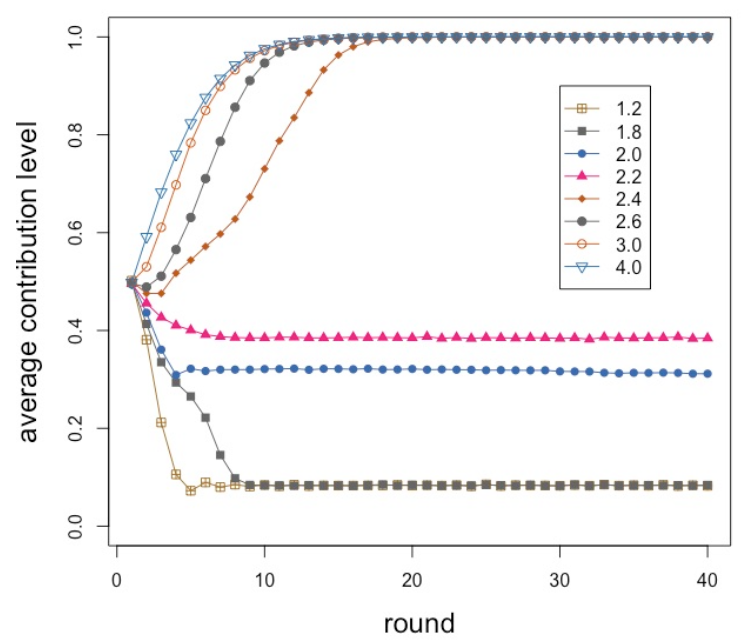
\includegraphics[width=\textwidth]{images/TAfig2_real.png}
    \caption{Figure 2 from \cite{RN49}. }
    \label{TAfig2_real}
  \end{subfigure}
  \hfill
  \begin{subfigure}[b]{0.45\textwidth}
    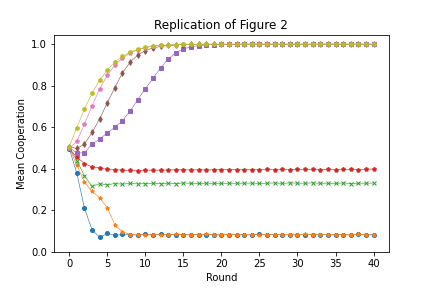
\includegraphics[width=1.25\textwidth]{images/TAfig2.png}
    \caption{Replication of \ref{TAfig2_real}. }
    \label{TAfig2}
  \end{subfigure}
  \caption{Comparison of reported results from \cite{RN49} and replicated results. Each series represents a value for the enhancement factor $r \in [1.2, 1.8, 2.0, 2.2, 2.4, 2.6, 3.0, 4.0]$, which corresponds to blue circles, orange stars, green crosses, red pentagons, purple squares, brown diamonds, pink pentagons, and olive hexagons respectively. They appear almost identical, indicating that the replication is successful.} \label{comp0}
\end{figure} 
\FloatBarrier

For further confirmation, Figures 5a and b from the paper were also replicated, shown in Figures \ref{comp1}, and \ref{comp2}. These correspond to modifying the underlying graph to a purely spatial ($\alpha = 0$), or preferential attachment ($\alpha = 1)$ model. The similarity of these results indicates both the agent and graph models correctly replicate the descriptions given in \cite{RN49}.

\FloatBarrier
\begin{figure}[!h] 
  \begin{subfigure}[b]{0.45\textwidth}
    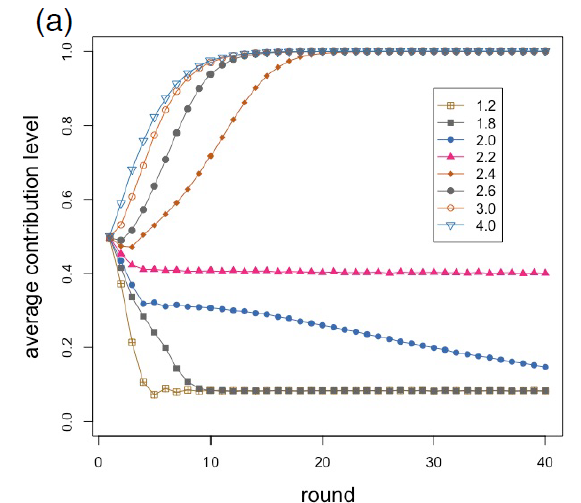
\includegraphics[width=\textwidth]{images/TAfig4a_real.png}
    \caption{Figure 5a from \cite{RN49}. $\alpha = 0$ }
    \label{TAfig4a_real}
  \end{subfigure}
  \hfill
  \begin{subfigure}[b]{0.45\textwidth}
    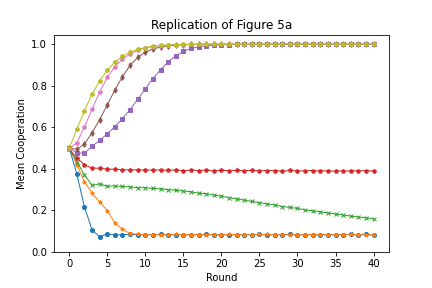
\includegraphics[width=1.35\textwidth]{images/TAfig4a.png}
    \caption{Replication of \ref{TAfig4a_real}. }
    \label{TAfig4a}
  \end{subfigure}
  \caption{Comparison of reported results from \cite{RN49} and replicated results. Each series represents a value for the enhancement factor $r \in [1.2, 1.8, 2.0, 2.2, 2.4, 2.6, 3.0, 4.0]$, which corresponds to blue circles, orange stars, green crosses, red pentagons, purple squares, brown diamonds, pink pentagons, and olive hexagons respectively. Once again, the replication is successful. } \label{comp1}
\end{figure} 
\FloatBarrier




\FloatBarrier
\begin{figure}[!h] 
  \begin{subfigure}[b]{0.45\textwidth}
    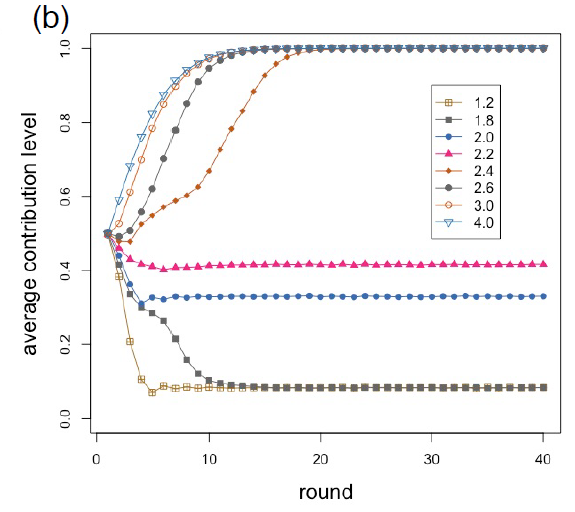
\includegraphics[width=\textwidth]{images/TAfig4b_real.png}
    \caption{Figure 5b from \cite{RN49}. $\alpha = 1$ }
    \label{TAfig4b_real}
  \end{subfigure}
  \hfill
  \begin{subfigure}[b]{0.45\textwidth}
    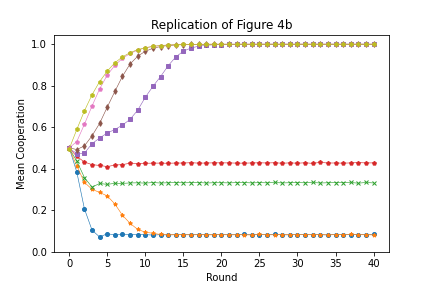
\includegraphics[width=1.35\textwidth]{images/TAfig4b.png}
    \caption{Replication of \ref{TAfig4b_real}. }
    \label{TAfig4b}
  \end{subfigure}
  \caption{Comparison of reported results from \cite{RN49} for $\alpha = 1$. Each series represents a value for the enhancement factor $r \in [1.2, 1.8, 2.0, 2.2, 2.4, 2.6, 3.0, 4.0]$, which corresponds to blue circles, orange stars, green crosses, red pentagons, purple squares, brown diamonds, pink pentagons, and olive hexagons respectively. } \label{comp2}
\end{figure} 
\FloatBarrier

They key results from \cite{RN49} have been reproduced. Other results from their paper, where the mean degree is varied, have also been reproduced, but are not included for the sake of brevity.\\


\section{Robustness}
The robustness of results was discussed qualititatively in \cite{RN49}, and the authors demonstrated consistency in results. However no quantitative analysis was provided. To examine the variance in the results, the number of trials, $T$ was increased to 120. The first plot examines the shape of the distribution for each of the series by plotting the empirical 2.5\% and 97.5\% quantiles. \\

\FloatBarrier
\graphCap{sensitivity2.png}{0.8}{2.5\% and 97.5\% quantiles for each series. Each series represents a value for the enhancement factor $r \in [1.2, 1.8, 2.0, 2.2, 2.4, 2.6, 3.0, 4.0]$, which corresponds to blue, orange, green, red, purple, brown, pink, and olive respectively. The mean is shown as a solid line, and the quartiles as dashed. Only 6 out of 120 trials lie outside the dashed lines for each series.}{sens2}
\FloatBarrier
The series corresponding to $r=2.2$ shows a 97.5\% quantile trend of around 0.58. This is much higher than the mean trend. This shows the influence of the particular network within the network model, particularly for the critical values at which cooperation is sustained but full cooperation is not achieved. It is interesting to note that this phenomenon does not occur for the $r=2$ line, which also achieves incomplete but non-zero cooperation. For $r \in [2.2, 2.28]$, the 2.5\% quantile is the same, however the mean trends are different. There appears to be a lower bound of 0.33, which represents a population switching between 0.25 and 0.5 similar to the lower bound of 0.0835 discussed in reference to \ref{comp0}. The image below applies the Central Limit Theorem to the cooperation level, and plots a $95\%$ confidence interval for the mean for each series. The Central Limit Theorem derives a 95\% CI for the mean, as $\pm 1.96*\frac{\sigma}{\sqrt{T}}$, where $\sigma$ is the empirical standard deviation. The Central Limit Theorem is applicable, as there are more than 30 samples for each series. \\
\FloatBarrier
\graphCap{sensitivity1.png}{0.8}{95\% Confidence interval for the mean of each series. Each series represents a value for the enhancement factor $r \in [1.2, 1.8, 2.0, 2.2, 2.4, 2.6, 3.0, 4.0]$, which corresponds to blue, orange, green, red, purple, brown, pink, and olive respectively. The mean is shown in the solid line, and the bounds of the confidence interval are shown as dashed lines. It is evident that the results are stable. Only the middle series, $r=2.2$, shows some variance.}{sens1}
\FloatBarrier
The image shows that the means are stable, and the results are robust. The confidence intervals for the mean are symmetric about the mean, due to the assumption of limiting normality. \\

To investigate the effect of network structure on cooperation, the Tomassini Antonioni model will be extended to other network models. \\

\section{Extension to Other Network Models}

In \ref{RG}, three main network models are discussed. These are the Erd\H{o}s--R\'enyi graph, \emph{small-world} network (WS), and also the Barab\'{a}si--Albert (BA) model. In the following analysis, $G(n,r)$ graphs are chosen for Erd\H{o}s--R\'enyi graphs, and denoted RRG (random regular graphs). This is to be able to control the mean degree. All three of these network models are implemented using the \verb+networkx+ Python package. For comparison, the model described by Tomassini and Antonioni in \cite{RN51} is included, and denoted Tomassini Antonioni Graph (TAG). \\

Small--world networks actually describe a family of graphs, depending on the parameter $p$. For this analysis, $p$ was set to 0.1, which preserves local clustering and reduces the average shortest path length. Importantly, only connected WS graphs are used. If the graph generated is not connected, then a new one with the same parameter is generated until they are connected. This is convention to allow strategies to propagate throughout the graph. \\

Similarly, TAG is a family of graphs. In the plots below, the proportion parameter $\alpha$ is set to 0.3, as recommended by \cite{RN49}. Firstly, a sample of 100 graphs for each model were taken, and their descriptive statistics were computed. \\


\FloatBarrier

    

\begin{table}[!h]
\begin{center}
\begin{tabular}{|l|l|l|l|l|}
\hline
Graph Type & Mean Degree & $l$ & $C_\Delta$ & Degree Variance \\ \hline
BA         & 5.96        & 3.24                         & 0.05                   & 40.80           \\ \hline
RRG        & 6           & 3.75                         & 0.01                   & 0               \\ \hline
TAG        & 5.99        & 3.84                         & 0.22                   & 16.95           \\ \hline
WS         & 6           & 5.39                         & 0.44                   & 0.57            \\ \hline
\end{tabular}
\caption{Computed characteristics for BA, RRG, TAG, and WS models. The characteristics were computed over 100 samples of each graph, and then averaged. } \label{graph_stats}
\end{center}
\end{table}

\FloatBarrier

The degree variance does not accurately describe all the facets of the degree distribution, so a histogram for each model is plotted below. For each graph model, 10 graphs were created according to the previously described parameters and their degree counts summed to create the histograms. \\
\FloatBarrier
\graphCap{hist1.png}{0.7}{Degree Histogram for WS and RRG models. The RRG model enforces a degree of 6 for every node. The WS model starts from a lattice, then rewires each link with probability $p$.}{hist1}
\FloatBarrier
\graphCap{hist2.png}{0.7}{Degree Histogram for BA and TAG models, on a logarithmic scale. The logarithmic scale clearly shows the counts for higher degrees. Because the TAG model uses preferential attachment only $\alpha = 0.3$ proportion of the time, it is not a true scale--free distribution. }{hist2}
\FloatBarrier
One of the goals of the TAG was to preserve a higher clustering coefficient than BA graphs, while remaining approximately scale--free. Table \ref{graph_stats} emphasises this effect. From these descriptive statistics, it appears that BA and RRG can be considered similar except for their degree distributions. The mean cooperation level for each graph was plotted. Because this is novel analysis, the number of trials $T$ was set to 80, and each trial observes 60 steps. \\

\FloatBarrier
\graphCap{graphs1.png}{0.8}{Comparing Models, $1.85 \leq r \leq 2.0$. In each graph, the blue, orange, green, red lines correspond to the WS model, TAG model, BA model, and RRG model respectively. For $r<1.85$, minimal cooperation is observed, so these plots are not shown. It is observed that first RRG, then BA, then TAG, then WS achieve non--trivial cooperation. This corresponds to the order of increasing $C_\Delta$. }{graphs11}
\FloatBarrier

It appears that $C_\Delta$ dictates the value for $r$ for which non--trivial cooperation is observed. Interestingly, for $\alpha = 0.3$, 30\% of the TAG graph are nodes added in BA style. Yet the TAG graph follows the trend of the WS model more than the BA model.
\FloatBarrier
\graphCap{graphs2.png}{0.8}{Comparing Graph models, $2.25\leq r \leq 2.4$. In each graph, the blue, orange, green, red lines correspond to the WS model, TAG model, BA model, and RRG model respectively. For $2.0<r<2.25$, the cooperation levels were very similar around 0.5, so the plots are not shown.  It is an almost perfect trend reversal, as WS is the first graph to achieve full cooperation, then TAG, then BA and finally RRG. For $r>2.4$, full cooperation was always achieved. \\ }{graphs1}
\FloatBarrier
For higher ranges of $r$, it is more interesting. The WS and TAG trends achieve full cooperation earlier. This seems to indicate that the agents are more uniform under this graph structure. The WS and TAG models have a small range of $r$ for which non--trivial cooperation is observed. These graph models also have high $C_\Delta$, which may propagate strategies through the population, and enforce homogeneity in contribution. Both the WS and RRG model have very low degree variance, yet behave quite differently. It appears that the degree distribution does not impact the cooperation level for Tomassini Antonioni style agents. \\

\section{Summary}

This chapter focussed exclusively on agents defined by Tomassini and Antonioni in \cite{RN49}. Tomassini and Antonioni demonstrated that these agents are a good proxy for human interactions, and simulated the Public Goods Game on a custom network model. These results were perfectly replicated, and both plots are shown in Figures \ref{comp0}, \ref{comp1}, \ref{comp2}.  A lower bound for cooperation of 0.0835 was demonstrated analytically. The robustness of these results were also examined. It is shown that 120 repetitions were sufficient to estimate the mean of each series, however the empirical quantile plots showed that there is quite high variance in distribution for the series corresponding to $r=2.2$.\\ 

The agents from this model were then tested on different models for random graphs. The results are interesting in the range $1.85\leq r \leq 2.4$. The trend indicates that models with high clustering coefficient $C_\Delta$ do not support intermediate levels of cooperation, and remain at the lower bound of cooperation for higher $r$ and full cooperation for lower $r$ relative to models with low $C_\Delta$. Other characteristics of the graph model, such as degree distribution and ASPL did not seem to have an effect. \\





\chapter{PGG on Graphs: Replicator Dynamics} 
\label{Chapter:Rep}
This chapter investigates the effect of network structure on observed cooperation for the linear PGG described in \ref{ToTC}. The first section uses a simple lottery game to demonstrate the implementation of replicator dynamics. To this end, the paper \cite{RN30} is replicated and extended. \\

Then replicator dynamics are applied to the linear PGG. Under this regime, it is found that graphs with a power--law degree size distribution exhibit higher cooperation, when controlling for mean degree $m$. It is hypothesised that nodes with low degree size cooperate more, and the family of power--law models are characterised by a large number of low--degree nodes, resulting in higher overall cooperation than the WS and RRG model. \\
\section{Proof of Concept: Replicator and Imitation Dynamics} \label{Lottery_Me}
\subsection{Outline}
The paper chosen to replicate imitation and replicator dynamics was \cite{RN30}, which models a two-stage lottery game. Refer to \ref{Lottery} for a description of the game and the strategy space $S$. \\

The paper implemented agent--based replicator $(\alpha = 1)$ and imitation $(\alpha = 0)$ dynamics. After each round, every agent $i$ randomly chooses another agent $j$ from the population, and calculates $q_i$, \\

\begin{equation} \label{rep}
q_i = \Bigg[ \frac{|\pi_j - \pi_i|}{\Delta} \Bigg]^\alpha \mathbbm{1}_{\{\pi_j>\pi_i\}}, \quad  0 \leq \alpha \leq 1.\end{equation} 

In the formulation, $\Delta$ scales the difference so that $0 \leq q_i \leq 1$, and $\Delta = 16$ in this two-stage lottery game. Each agent then changes from strategy $i$ to strategy $j$ if $q_i \geq r_i,$ $r_i \sim \mathsf{U}(0,1)$. \\

\subsection{Results Comparison}
The simulated results were compared to the paper for $\alpha = 0, 1, 0.5$, and are shown below. \\

\FloatBarrier 
\begin{figure}[!h]
  \begin{subfigure}[b]{0.45\textwidth}
    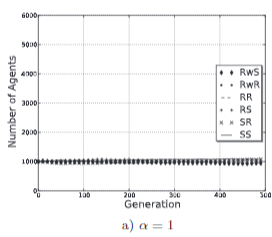
\includegraphics[width=\textwidth]{images/lottery1.png}
    \caption{Figure 5a from \cite{RN30}. The strategies SS, RR, SR, RS, R--WR, R--WS are represented by a solid line, crosses, plusses, dashes, dots and diamonds respectively. }
    \label{lottery1}
  \end{subfigure}
  \hfill
  \begin{subfigure}[b]{0.45\textwidth}
    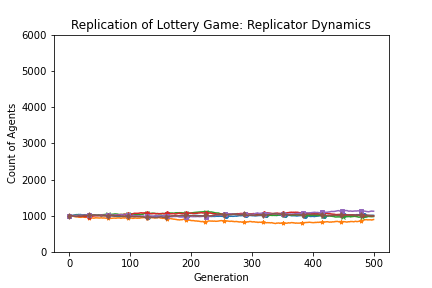
\includegraphics[width=1.25\textwidth]{images/lottery1_me.png}
    \caption{Replication of \ref{lottery1}. The strategies SS, RR, SR, RS, R--WR, R--WS are represented by blue circles, orange stars, green crosses, red pentagons, brown diamonds, and purple squares respectively.}
    \label{lottery1_me}
  \end{subfigure}
  \caption{Replication of Figure 5a from \cite{RN30}. The replication is successful, but these conditions do not provide anything interesting regarding replicator dynamics. Because the expected value of the strategies are equal, no strategy has an evolutionary advantage over any other.} \label{lottery_comp0}
\end{figure} 
\FloatBarrier

\FloatBarrier 
\begin{figure}[!h]
  \begin{subfigure}[b]{0.45\textwidth}
    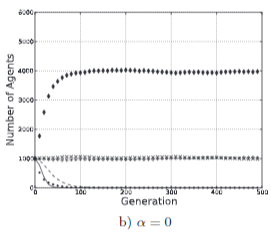
\includegraphics[width=\textwidth]{images/lottery2.png}
    \caption{Figure 5b from \cite{RN30}. The strategies SS, RR, SR, RS, R--WR, R--WS are represented by a solid line, crosses, plusses, dashes, dots and diamonds respectively. }
    \label{lottery2}
  \end{subfigure}
  \hfill
  \begin{subfigure}[b]{0.45\textwidth}
    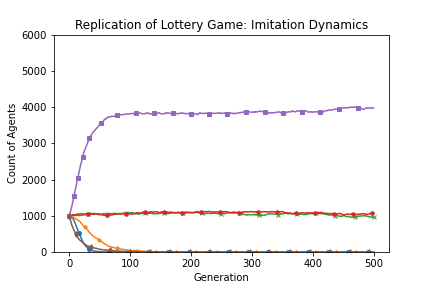
\includegraphics[width=1.25\textwidth]{images/lottery2_me.png}
    \caption{Replication of \ref{lottery2}. The strategies SS, RR, SR, RS, R--WR, R--WS are represented by blue circles, orange stars, green crosses, red pentagons, brown diamonds, and purple squares respectively.}
    \label{lottery2_me}
  \end{subfigure}
  \caption{Replication of Figure 5b from \cite{RN30}. The results are well replicated, and this model for imitation dynamics can be explored on other games.} \label{lottery_comp1}
\end{figure} 
\FloatBarrier



\FloatBarrier 
\begin{figure}[!h]
  \begin{subfigure}[b]{0.45\textwidth}
    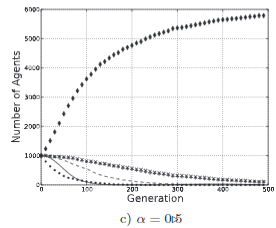
\includegraphics[width=\textwidth]{images/lottery3.png}
    \caption{Figure 5c from \cite{RN30}. The strategies SS, RR, SR, RS, R--WR, R--WS are represented by a solid line, crosses, plusses, dashes, dots and diamonds respectively. }
    \label{lottery3}
  \end{subfigure}
  \hfill
  \begin{subfigure}[b]{0.45\textwidth}
    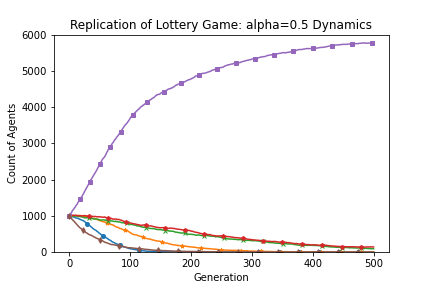
\includegraphics[width=1.25\textwidth]{images/lottery3_me.png}
    \caption{Replication of \ref{lottery3}. The strategies SS, RR, SR, RS, R--WR, R--WS are represented by blue circles, orange stars, green crosses, red pentagons, brown diamonds, and purple squares respectively. }
    \label{lottery3_me}
  \end{subfigure}
  \caption{Replication of Figure 5c from \cite{RN30}. This is neither true imitation or replicator dynamic, but provides an intermediary case.} \label{lottery_comp2}
\end{figure} 
\FloatBarrier


 It is also interesting to examine the results when the lottery win probability $p$ is not 0.5. For replicator dynamics, the strategy with the highest expected value eventually wins out, but for imitation dynamics the result is not so obvious. This was shown in Figure 6 from \cite{RN30}, and replicated below. For $p=0.4$, the expectation--maximising strategy is SS, but R--WS has an evolutionary advantage and takes over the population. This is supported by theoretical results in \cite{RN30}. Similarly, for $p=0.55$, the expectation--maximising strategy is RR, but R--WS also takes over the population. \\
 
 \FloatBarrier 
\begin{figure}[!h]
  \begin{subfigure}[b]{0.45\textwidth}
    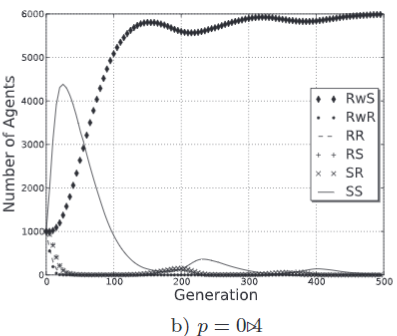
\includegraphics[width=\textwidth]{images/lotteryp4.png}
    \caption{Figure 6b from \cite{RN30}. The strategies SS, RR, SR, RS, R--WR, R--WS are represented by a solid line, crosses, plusses, dashes, dots and diamonds respectively.}
    \label{lotteryp4}
  \end{subfigure}
  \hfill
  \begin{subfigure}[b]{0.45\textwidth}
    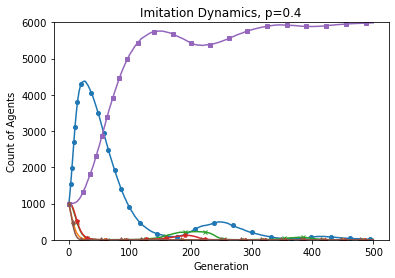
\includegraphics[width=1.25\textwidth]{images/lotteryp4_me.png}
    \caption{Replication of \ref{lotteryp4}. The strategies SS, RR, SR, RS, R--WR, R--WS are represented by blue circles, orange stars, green crosses, red pentagons, brown diamonds, and purple squares respectively. }
    \label{lotteryp4_me}
  \end{subfigure}
  \caption{Replication of Figure 6b from \cite{RN30}. Although SS is the expectation--maximising strategy, it is not an ESS, and R--WS has the evolutionary advantage.} \label{lottery_comp4}
\end{figure} 
\FloatBarrier

 \FloatBarrier 
\begin{figure}[!h]
  \begin{subfigure}[b]{0.45\textwidth}
    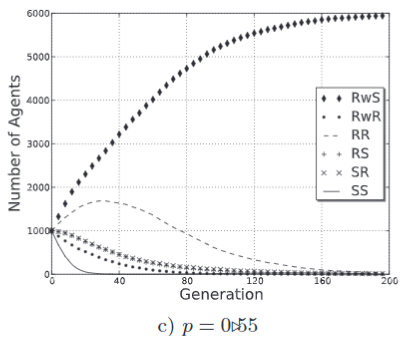
\includegraphics[width=\textwidth]{images/lotteryp055.png}
    \caption{Figure 6c from \cite{RN30}. The strategies SS, RR, SR, RS, R--WR, R--WS are represented by a solid line, crosses, plusses, dashes, dots and diamonds respectively.}
    \label{lotteryp055}
  \end{subfigure}
  \hfill
  \begin{subfigure}[b]{0.45\textwidth}
    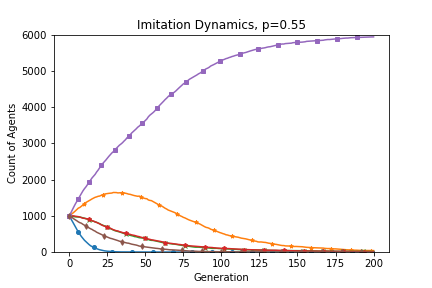
\includegraphics[width=1.25\textwidth]{images/lotteryp055_me.png}
    \caption{Replication of \ref{lotteryp055}. The strategies SS, RR, SR, RS, R--WR, R--WS are represented by blue circles, orange stars, green crosses, red pentagons, brown diamonds, and purple squares respectively. }
    \label{lotteryp4_me_2}
  \end{subfigure}
  \caption{Replication of Figure 6c from \cite{RN30}. In this case, RR is expectation--maximising, but R--WS still takes over the population.} \label{lottery_comp5}
\end{figure} 
\FloatBarrier

\subsection{Extension}
In \cite{RN30}, plots for $p=0.3, 0.7$ were also shown, however the expectation--maximising strategies win out quickly, so they are not included here. It is notable that in Figure \ref{lotteryp4_me}, there are some fluctuations that occur before stability. This is investigated further. \\

Consider the three strategies RS, SS, R--WS under the $p=0.4$ regime. For simplicity, assume these three strategies complete the strategy space. Their distributions are shown below. \\
\begin{align*}
    \mathbb P_{\text{RS}}(x = \pi)  &= \begin{cases} 0.4 \quad \pi = 12 \\
    0.6 \quad \pi =4 
    \end{cases}, \\
        \mathbb P_{\text{R--WS}}(x = \pi)  &= \begin{cases} 0.4 \quad \pi = 12 \\
    0.24 \quad \pi =8 \\
    0.36 \quad \pi = 0\\
    \end{cases}, \\
    \mathbb P_{\text{SS}}(x = \pi)  &= \mathbbm{1}_{\pi = 8}.
\end{align*}
Under imitation dynamics, a strategy $i$ has an evolutionary advantage over $j$, $j \prec i$, if $\mathbb P(\pi_i > \pi_j) > \mathbb P(\pi_i < \pi_j)$. In the example above, RS $\prec$ SS $\prec$ R--WS $\prec$ RS, which is a cycle. In \ref{lotteryp4_me}, the strategy SS eliminates RS much faster than RS can eliminate R--WS, so SS temporarily grows, and then succumbs to R--WS. \\

This relationship can be expressed as as a set of difference equations. Call $\rho_{\text{RS},t}, \rho_{\text{R--WS},t}, \rho_{\text{SS},t}$ the proportion of each strategy present at time $t$. The boundary condition is $\rho_{\text{RS},t}+ \rho_{\text{R--WS},t}+ \rho_{\text{SS},t} = 1$, $\forall t \in [0,T]$. Denote $\mathcal F_t$ the natural filtration of $\rho_{\text{RS},t}, \rho_{\text{R--WS},t}, \rho_{\text{SS},t}$ at time $t$.  \\
\begin{align*}
    \mathbb E \big [\rho_{\text{RS},t+1}| \mathcal F_t \big ] &= \rho_{\text{RS},t} \Bigg [ \rho_{\text{R--WS},t} [\mathbb P (\pi_\text{RS} > \pi_{\text{R--WS}}) -\mathbb P (\pi_\text{RS} < \pi_{\text{R--WS}}) ] \\
    &+ \rho_{\text{SS},t} [\mathbb P (\pi_\text{RS} > \pi_{\text{SS}}) -\mathbb P (\pi_\text{RS} < \pi_{\text{SS}}) ] \Bigg ] \\
    &= \rho_{\text{RS},t}\Bigg [ \rho_{\text{R--WS},t}(0.456 - 0.396) + \rho_{\text{SS},t}(0.4 - 0.6)  \Bigg ] \\
    &= \rho_{\text{RS},t}\Bigg [ \rho_{\text{R--WS},t}(0.06) + \rho_{\text{SS},t}(-0.2)  \Bigg ]
\end{align*}
The same logic can be applied for the difference equations for$\rho_{\text{SS},t}, \rho_{\text{R--WS},t}$. \\
\begin{align*}
    \mathbb E \rho_{\text{R--WS},t+1} &= \rho_{\text{R--WS},t} \Bigg [ \rho_{\text{RS},t} [\mathbb P (\pi_\text{R--WS} > \pi_{\text{RS}}) -\mathbb P (\pi_\text{R--WS} < \pi_{\text{RS}}) ] \\
    &+  \rho_{\text{SS},t} [\mathbb P (\pi_\text{R--WS} > \pi_{\text{SS}}) -\mathbb P (\pi_\text{R--WSS} < \pi_{\text{SS}}) ] \Bigg ] \\
    &= \rho_{\text{R--WS},t}\Bigg [ \rho_{\text{RS},t}(0.396-0.456) + \rho_{\text{SS},t}(0.4 - 0.36)  \Bigg ] \\
    &= \rho_{\text{R--WS},t}\Bigg [ \rho_{\text{RS},t}(-0.06) + \rho_{\text{SS},t}(0.04)  \Bigg ] \\
    \mathbb E \rho_{\text{SS},t+1}&= \rho_{\text{SS},t}\Bigg [ \rho_{\text{RS},t}(0.2) + \rho_{\text{R--WS},t}(-0.04)  \Bigg ]
\end{align*}
This set of difference equations cannot be solved analytically, and the numerical simulation is the same as Figure \ref{lotteryp4_me}. Under imitation dynamics, once a strategy is eliminated it can never return, and the elimination of RS ensures the eventual dominance of R--WS. RS is eliminated because it has the highest pairwise death rate, as SS dominates it with a rate of 0.2. This is much larger than any other pairwise comparison rate.  \\

The difference equations have ignored the effect of the other strategies, as they are negligible, but they were included for simulation. The image in \ref{lotteryp4_me} is aggregated over 20 trials, and the time to elimination is quite variable. The empirical quantiles are shown below, instead computed over 120 trials.  \\

\FloatBarrier
\graphCap{lotteryp4_me_quantiles_empirical.png}{0.75}{Empirical 2.5\%, 97.5\% Quantiles of Imitation Dynamics Lottery Game, $p=0.4$, T = 120. The strategies SS, RR, SR, RS, R--WR, R--WS are represented by blue circles, orange stars, green crosses, red pentagons, brown diamonds, and purple squares respectively. The quantile for each series is the dashed line. }{lottery_quantiles_empirical}
\FloatBarrier
Figure \ref{lottery_quantiles_empirical} shows how great the variance of certain series are, particularly SS and R--WS. When R--WS is prominent and the strategies SR, RS are not extinct, SR, RS are able to grow. This occurs around the 200th generation. The strategy SS, which outperforms SR and RS, then dominates them. SS is dominated by R--WS, and this cycle continues until SR and RS are eliminated. The reason that they are eliminated is because the highest rate of dominance is SS over SR, RS. \\
\FloatBarrier
\graphCap{lotteryp4_me_quantiles.png}{0.75}{95\% Confidence Interval for the Mean, Imitation Dynamics Lottery Game, $p=0.4$, T = 120. The strategies SS, RR, SR, RS, R--WR, R--WS are represented by blue circles, orange stars, green crosses, red pentagons, brown diamonds, and purple squares respectively. The confidence interval for each series is the dashed line. }{lottery_quantiles}
\FloatBarrier
 The computed confidence intervals assume a normal distribution of the mean under the Central Limit Theorem. The computed standard deviation of each point in the time series is used as an estimate of the true standard deviation. Because the number of trials $T=120$, the confidence interval is tight around the sample mean. The original paper uses $T=20$, which results in a confidence interval four times as wide Figure \ref{lottery_quantiles}. Therefore it is suggested that more than 20 trials are used for future samples. \\



\subsection{Summary}
The purpose of replicating \cite{RN30} was to demonstrate replicator and imitation dynamics. This demonstration was achieved, and now these dynamics can be applied to the PGG. A cycle of strategies was demonstrated for imitation dynamics under a $p=0.4$ regime. Although the original paper did not investigate the distribution of results, they are discussed above. The paper \cite{RN30} did not use an underlying network structure, but the dynamics can easily be transposed onto a graph by limiting the sample space of agents to neighbours. \\


\section{Local Replicator Dynamics for Public Good Games}
\subsection{Outline}
The following section investigates the effect of graph model on cooperation under local replicator dynamics. The graph models from \ref{other_networks} are also investigated here, and sample characteristics are given in Table \ref{graph_stats}. The game is played by a population of 500 agents, where each agents hosts a play of the PGG with their neighbours. After every agent has hosted, the agent--based replicator dynamics from equation \eqref{rep} are implemented for each agent. Each plot aggregates the mean of each series over 80 trials. \\

It is found that the graphs with a power--law degree size distribution induce higher cooperation. The effect of $C_\Delta$ is isolated under a power--law degree size distribution by using a new model type, PL, and is also examined in the WS family of graph models. Under the PL model, higher $C_\Delta$ weakly induces higher cooperation, while the trend is reversed for the WS family of models. \\

Then the effect of targeted mean degree $m$ is examined for RRG and BA models. Both of these experiments indicate that higher $m$ lead to lower cooperation. Finally, the cooperation levels are stratified by degree size within a BA graph model. This experiments shows that the nodes with low degree size have a higher contribution proportion than average, which may explain the trend. \\

\subsection{Results}
These results examine the effect of network model on cooperation. For consistency, the WS model has parameter $p=0.1$ and the TAG model has parameter $\alpha = 0.3$, which aligns with Chapter \ref{TA}. Replicator dynamics result in slower convergence than the satisfaction model in Chapter \ref{TA}. Therefore the number of generations has been extended to 200, so that equilibrium is observed. Figure \ref{replicator_low} shows the TAG and BA model inducing higher cooperation than WS, RRG models. This trend continues for $2.5 \leq r \leq 7.5$. It appears that graph models with a power law degree size distribution induce higher cooperation. The results discussed in Chapter \ref{Chapter:Lit} corroborate this trend. \\
\FloatBarrier
\graphCap{replicator_graphs_low.png}{0.8}{Comparing Graph Models: Replicator Dynamics. Trend for $r \in \{2, 2.5, 3, 3.5\}$. In each graph, the blue circles, orange stars, green crosses, and red pentagons correspond to the WS model, TAG model, BA model, and RRG model respectively. }{replicator_low} 
\FloatBarrier
\graphCap{replicator_graphs_medium}{0.8}{Comparing Graph Models: Replicator Dynamics. Trend for $r \in \{4,4.5,5,5.5\}$. In each graph, the blue circles, orange stars, green crosses, and red pentagons correspond to the WS model, TAG model, BA model, and RRG model respectively. }{replicator_medium}
\FloatBarrier
\graphCap{replicator_graphs_large}{0.8}{Comparing Graph Models: Replicator Dynamics. Trend for $r \in \{6,6.5,7,7.5\}$. In each graph, the blue circles, orange stars, green crosses, and red pentagons correspond to the WS model, TAG model, BA model, and RRG model respectively. }{replicator_large}\FloatBarrier



There is insufficient information to determine if the clustering coefficient $C_\Delta$ influences cooperation, because the graph models are too varied. Therefore, it will need to be tested in isolation.\\

\subsection{Isolating the Effect of Clustering Coefficient: Power Law Degree Size Distribution}
To test the hypothesis that the average clustering coefficient $C_\Delta$ does not impact cooperation, the \verb+power_law+ model was used to create another graph model, denoted PL. It induces a degree distribution with power law shape, but the parameter $p$ dictates the clustering coefficient. After each node is connected, the parameter $p$ determines the probability that the next link joins two neighbours, completing the triangle. Two degree histograms are plotted below, which emphasise the degree size distribution. \\
\FloatBarrier
\graphCap{PL01BA.png}{0.5}{Comparison of Power Law Clustering Graph with BA model, $p=0.1$. The degree histograms are similar, so the only difference is the clustering coefficient.}{PL01BA}
\FloatBarrier
\graphCap{PL05BA.png}{0.5}{Comparison of Power Law Clustering Graph with BA model, $p=0.5$. The degree histograms are similar, so the only difference is the clustering  coefficient.}{PL05BA}
\FloatBarrier
The summary statistics are also reported. It is important to note the only statistic that noticeably changes is $C_\Delta$, as desired. \\
\FloatBarrier
\begin{table}[!h]
\begin{center}
\begin{tabular}{|l|l|l|l|l|}
\hline
Graph Type & Mean Degree & $l$ & $C_\Delta$ & Degree Variance \\ \hline
PL: $p=0.1$        & 5.96        & 3.234                         & 0.10                   & 42.35           \\ \hline
PL: $p=0.2$        & 5.96           & 3.24                         & 0.15                   & 44.07               \\ \hline
PL: $p=0.3$       & 5.96        & 3.23                       & 0.20                   & 46.28           \\ \hline
PL: $p=0.4$       & 5.96        & 3.25                         & 0.25                   & 47.92           \\ \hline
PL: $p=0.5$         & 5.96           & 3.26                         & 0.30                   & 50.47            \\ \hline
\end{tabular}
\caption{Computed characteristics for PL graph, varying cluster parameter $p$. The characteristics were computed over 100 samples of each graph, and then averaged. } \label{graph_stats}
\end{center}
\end{table}
\FloatBarrier
\graphCap{comparing_power_p_low.pdf}{0.8}{To test the effect of $C_\Delta$, the parameter $p$ in a PL graph was varied. In each graph, the blue circles, orange stars, green crosses, red pentagons, and purple squares correspond to $p=[0.1,0.2,0.3,0.4,0.5]$ respectively. The observed trend is that higher $C_\Delta$ leads to marginally higher cooperation.}{power_p_low}
\FloatBarrier
\graphCap{comparing_power_p_high.pdf}{0.8}{To test the effect of $C_\Delta$, the parameter $p$ in a PL graph was varied. In each graph, the blue circles, orange stars, green crosses, red pentagons, and purple squares correspond to $p=[0.1,0.2,0.3,0.4,0.5]$ respectively. The trend is unclear here, because $r=2.75, 3.5$ indicate higher $C_\Delta$ leads to higher cooperation, but that trend is not observed in for $r=3.0,3.25$.}{power_p_high} \FloatBarrier

These tests indicate that, when controlling for degree size distribution, the clustering coefficient $C_\Delta$ may have a marginal effect. The correlation is weakly positive, and is much more evident for $1.75\leq r\leq 3.0$. It is also necessary to test the effect of $C_\Delta$ under a different degree size distribution. \\

\subsection{Isolating the Effect of Clustering Coefficient: Constant Degree Size Distribution}
The WS model is a family of graphs, characterised by rewiring probability $p$. By increasing $p$, the $l$ statistic is reduced while $C_\Delta$ remains high for $0\leq p\leq0.15$. However there exists a region for $p$ where $C_\Delta$ decreases and $l$ does not change as rapidly. It is this region that will be isolated to test the effect of local clustering on cooperation in graphs under a near--constant degree distribution regime. Recall that a WS graph starts with a circle of nodes, each node connected to its adjacent $\frac{m}{2}$ circular neighbours. Hence the initial degree is $m$ for each node, and this only varies marginally due to $p$. There are certainly no scale factors such as in the PL, BA, or TAG models. \\

\FloatBarrier
\begin{table}[!h]
\begin{center}
\begin{tabular}{|l|l|l|l|l|}
\hline
Graph Type & Mean Degree & $l$ & $C_\Delta$ & Degree Variance \\ \hline
WS: $p=0.1$        & 6        & 5.41                         & 0.44                  & 0.57           \\ \hline
WS: $p=0.2$        &6           & 4.53                         & 0.316                   & 1.06               \\ \hline
WS: $p=0.3$        &6           & 4.16                         & 0.22                   & 1.51               \\ \hline
WS: $p=0.4$       & 6        & 3.95                         & 0.14                  & 1.93           \\ \hline
WS: $p=0.5$         & 6           & 3.83                         & 0.09                   & 2.25            \\ \hline
\end{tabular}
\caption{Computed characteristics for WS graph, varying rewiring probability parameter $p$. The characteristics were computed over 100 samples of each graph, and then averaged. } \label{graph_stats_WS}
\end{center}
\end{table}
\FloatBarrier

\graphCap{graph_p_med.pdf}{0.8}{Effect of rewiring $p$ in a WS model. In each graph, the blue circles, orange stars, green crosses, red pentagons, and purple squares correspond to $p=[0.1,0.2,0.3,0.4,0.5]$ respectively. The trend indicates that higher $p$ leads to higher cooperation.}{graph_p_med}
\FloatBarrier
\graphCap{graph_p_high.png}{0.8}{Capt. In each graph, the blue circles, orange stars, green crosses, red pentagons, and purple squares correspond to $p=[0.1,0.2,0.3,0.4,0.5]$ respectively. The same trend is observed here.}{graph_p_high}
\FloatBarrier
Figures \ref{graph_p_med} and \ref{graph_p_high} indicate that higher rewiring probability $p$ leads to higher cooperation. This indicates that lowering the clustering coefficient induces higher cooperation, a contradiction to Figures \ref{power_p_low} and \ref{power_p_high}. In those figures, there was a weak positive correlation between $C_\Delta$ and cooperation. At this stage, there is no feasible explanation for this discrepancy, so further investigation is required. \\

\subsection{The Effect of Mean Degree: RRG}
The initial experiments indicated that graphs with a power law degree distribution induced higher cooperation. This may be because they include nodes with higher degree. It is of interest to isolate the effect of higher degree on cooperation. To do this, a family of RRG are sampled, and the mean degree is varied between 4 and 8. \\


\graphCap{RRG_graph_m_med.pdf}{0.8}{The effect of mean degree, RRG model. In each graph, the blue circles, orange stars, green crosses, red pentagons, and purple squares correspond to $m =  [4,6,8,10,12]$ respectively. }{graph_m_low} \FloatBarrier

\graphCap{RRG_graph_m_high.pdf}{0.8}{The effect of mean degree, RRG model. In each graph, the blue circles, orange stars, green crosses, red pentagons, and purple squares correspond to $m =  [4,6,8,10,12]$ respectively. }{graph_m_med} \FloatBarrier

The plots above dissect the effect of increasing average degree across the whole graph. The trend is that higher degree leads to less cooperation. This trend is consistent across $3.0\leq r\leq6.5$. This indicates that the trend observed in Figure \ref{replicator_low} is not due to the power--law graphs having some nodes with higher degree, but must be explained in a different manner. These results can also be tested on a BA model. \\
\FloatBarrier
\graphCap{BA_graph_m_low.pdf}{0.8}{The effect of mean degree, BA model. In each graph, the blue circles, orange stars, green crosses, red pentagons, and purple squares correspond to $m = [4,6,8,10,12]$ respectively.}{BA_graph_m_low}
\FloatBarrier
\graphCap{BA_graph_m_med.pdf}{0.8}{The effect of mean degree, BA model. In each graph, the blue circles, orange stars, green crosses, red pentagons, and purple squares correspond to $m = [4,6,8,10,12]$ respectively.}{BA_graph_m_med}
\FloatBarrier
Across Figures \ref{graph_m_low}, \ref{graph_m_med},\ref{BA_graph_m_low}, and \ref{BA_graph_m_med} there is a consistent trend that higher targeted mean degree $m$ leads to lower cooperation. A plausible explanation is the \emph{scaled effect} of $r$. For an agent $i$ hosting a game of size $|N_i|$ with each agent defecting, then $\lceil \frac{|N_i|}{r}\rceil$ can be viewed as the number of agents who must start cooperating to ensure cooperation is the most profitable strategy. This is increasing in $|N_i|$, which lends credence to the hypothesis that lower degrees have a higher proportion of cooperators. It is also feasible that a node with low degree can be surrounded by cooperators, and become \emph{immune} to defection much faster than a high--degree node. This trend is very consistent across both models and varying $r$. \\

It also suggests that the increase in cooperation of the power--law graphs observed in Figures \ref{replicator_low}, \ref{replicator_medium}, and \ref{replicator_large} is not due to the high--degree nodes, but instead occurs because there exist a large proportion of nodes with degree lower than the common $m$.  \\

The last effect to consider is stratifying the nodes by degree within a single graph model. To do this, the BA model was used, and the cooperation level recorded for each nodes, then aggregated by degree. \\

\subsection{Cooperation Level Within a Single Graph Instance: BA model }
This experiment seeks to stratify the cooperation level of each point according to its degree. Earlier experiments indicated that increasing the targeted mean degree $m$ reduces cooperation, but that was measuring the whole--model cooperation. Instead, $m, r$ are fixed, and the cooperation level at the final step for each node is examined, and then aggregated over all nodes with that degree. This experiment necessitated reducing the mean degree, $m$ to 4, to reduce the range for degree size and therefore the number of trials required. Also, degree sizes with less than 5 representations across all trials were removed, as there is insufficient data. The number of trials, $T$, was set to 1000 to ensure the data was representative of the underlying mechanism. \\
\FloatBarrier
\graphCap{BA_degree_groups_20_1000_trimmed_4.pdf}{0.8}{Cooperation vs Node Degree: BA Model, $r=2.0$, $m=4$. The bar chart, plotted on the left axis, is a histogram of the degree size. On the right axis, and plotted in black, is the final cooperation level of all nodes according to their degree. The mean cooperation is plotted as red horizontal line, for comparison. }{BA_groups_low}
\FloatBarrier

\FloatBarrier
\graphCap{BA_degree_groups_45_1000_trimmed_4.pdf}{0.8}{Cooperation vs Node Degree: BA Model, $r=4.5, m =4$. The bar chart, plotted on the left axis, is a histogram of the degree size. On the right axis, and plotted in black, is the final cooperation level of all nodes according to their degree. The mean cooperation is plotted as red horizontal line, for comparison. }{BA_groups_med}
\FloatBarrier

\textbf{ADD IN M=6 HERE}
These figures demonstrate that the lower degree nodes contribute a greater fraction than the mean. The higher nodes are incentivised to defect, as their gain from defection can be very high. It is notable that this strategy does not propagate well, and even for low $r$ high cooperation is achieved. These results corroborate the findings in Figures \ref{BA_graph_m_low} and \ref{BA_graph_m_med}, which show that there is higher cooperation amongst lower degrees. \\

\subsection{Summary}
Four graph models were examined under replicator dynamics, and the results are plotted in Figures \ref{replicator_low}, \ref{replicator_medium}, and \ref{replicator_large}. The trend of these plots was that the models with power--law degree size distribution, specifically the BA and TAG models, induced higher cooperation. In an attempt to explain these results, several more experiments were carried out. \\

Firstly, the effect of $C_\Delta$ was examined for both a power--law graph (PL), and also the WS family of models. These produced weakly contradictory results. Under the WS model, increasing $C_\Delta$ reduced cooperation. Under the PL model, it was more unclear but it appears that increasing $C_\Delta$ weakly increases cooperation. At this stage, there is no explanation for these effects. \\

Then the effect of targeted mean degree $m$ was examined. This produced strong results across both the BA and RRG models, demonstrating that mean degree is negatively correlated to cooperation level. This gives some suggestion for the trends observed in Figures \ref{replicator_low}, \ref{replicator_medium}, and \ref{replicator_large}. Because the BA and TAG model have a power--law degree size distribution with the same mean degree $m$ as the WS, RRG models, they necessarily have a lot of nodes with degree less than $m$. These nodes cooperate more often than their higher degree size counterparts, so induce higher mean cooperation. 

\chapter{PGG on Graphs: Imitation Dynamics} 
\label{Chapter:ID}
\section{Local Imitation Dynamics for Public Good Games}
\subsection{Outline}
\subsection{Results}
\FloatBarrier
\graphCap{ID_low_gtype.pdf}{0.7}{Comparing Graph Models: Replicator Dynamics. Trend for $r \in \{4.0, 4.25, 4.5, 4.75\}$. In each graph, the blue circles, orange stars, green crosses, and red pentagons correspond to the WS model, TAG model, BA model, and RRG model respectively. It appears that the BA model induces the highest cooperation, then the TAG, followed by WS and RRG respectively. Observed cooperation correlates with degree size variance. It is interesting that the BA trend for $r=4.75$ is lower than the trend for $r=4.5$. This may be due to sampling variation. }{replicator_low} 
\FloatBarrier
\graphCap{ID_med_gtype.pdf}{0.7}{Comparing Graph Models: Replicator Dynamics. Trend for $r \in \{5.0, 5.25, 5.5, 5.75\}$. In each graph, the blue circles, orange stars, green crosses, and red pentagons correspond to the WS model, TAG model, BA model, and RRG model respectively. For $r\geq 5.5$, the TAG model induces the highest cooperation.}{replicator_medium}
\FloatBarrier
\graphCap{ID_high_gtype.pdf}{0.7}{Comparing Graph Models: Replicator Dynamics. Trend for $r \in \{6,6.5,7,7.5\}$. In each graph, the blue circles, orange stars, green crosses, and red pentagons correspond to the WS model, TAG model, BA model, and RRG model respectively. The TAG and RRG models overtake the BA model, while the WS model consistently induces the lowest cooperation amongst models. }{replicator_high}\FloatBarrier


\chapter{Conclusion} \label{Conclusion}
\section{Summary and Discussion} 
Chapter \ref{Chapter:Lit} defines classical game theory and explores the expansion to evolutionary game theory, and then to evolutionary game theory on graphs. There is a section on random graphs as models for social networks, which informs the choice of random graph models for the simulations. Ssection \ref{Simple} contains a lemma which motivates the inclusion of a graph structure for EGT analysis of the linear PGG. Without a graph structure, full defection is the only possible equilibrium, and no further analysis is required. Finally, there is a review of the current literature on PGG on graphs. The reference \cite{RN49} serves as a starting point for simulation in Chapter \ref{TA}. \\

From Chapter \ref{Chapter:Lit}, four graph models are chosen for simulation. These are the WS model, with rewiring $p=0.1$, the TAG model, with proportion parameter $\alpha=0.3$, the BA model, and the RRG model. The value of each parameter is taken from suggestions in the literature. Each model has targeted mean degree $m=6$, and $n=500$ nodes in Chapter \ref{TA} and $n=100$ afterwards.This discrepancy is due to constraints on simulation time. The true mean degree is a random variable under the TAG and BA model, however Table \ref{graph_stats} shows that the targeted mean degree is well approximated. Each of the WS, TAG, and BA model serve as models for social networks, but are quite different in clustering coefficient $C_\Delta$ and distribution of degree size. The literature does not recommend using RRG as a model for social networks, but it is included as a control. The RRG model can be considered as the least clustered model with constant degree size. The purpose of its inclusion is to provide data for an unclustered model, even though real-world social networks are generally well-clustered. \\


In Chapter \ref{TA}, the model proposed by Tomassini and Antonioni in \cite{RN49} is successfully replicated and then analysis is extended to examine the robustness of results, as well as the effect of different random graph models. The game is the linear PGG, but the agent model is a payoff satisfaction model, as opposed to an EGT model. The purpose of the payoff satisfaction model is to recreate decisions made by humans in a laboratory environment. Under the payoff satisfaction model, it is found that graph models with high clustering coefficient $C_\Delta$ enforce conformity in contribution, regardless of the distribution of degree size. That is, relative to models with a lower $C_\Delta$, high $C_\Delta$ graph models induce lower contribution in a low $r$ regime and higher contribution in a high $r$ regime. This is because agents are more successful in influencing their neighbours, and conformity is the result of high $C_\Delta$. \\

In Chapter \ref{Chapter:Rep}, simulation of replicator dynamics is introduced. Firstly, the paper \cite{RN30} is replicated and extended. The paper involves a lottery game described in Section \ref{Lottery}. The paper was chosen for its simple implementation of replicator dynamics, and it was successfully replicated. This provides authority to the simulations in Chapter \ref{Chapter:Rep} and Chapter \ref{Chapter:ID}. After the lottery paper is investigated, replicator dynamics are transposed to the linear PGG on random graphs. It is found that the random graph models with high degree size variance induce higher contribution. To explain this phenomenon, several further simulations are carried out. The effect of the rewiring parameter $p$ in the WS model on contribution are examined. A new model, the PL model, is introduced to examine the effects of $C_\Delta$ in a power-law degree distribution environment. These results indicate that degree size variance, as opposed to $C_\Delta$, is responsible for the difference in contribution level. A possible explanation is the high proportion of low degree nodes, which are readier to contribute. It is shown that lower mean degree $m$ results in higher contribution, so it is feasible that graph models with a high proportion of low degree nodes induce higher contribution.  \\

Chapter \ref{Chapter:ID} compares the graph models under imitation dynamics. Imitation dynamics use the same replicator equation \eqref{rep}, instead with $\alpha=0$. This enforces faster strategy switching, and the time to equilibrium is quicker for imitation than replicator dynamics. The same simulations from Chapter \ref{Chapter:Rep} are run in Chapter \ref{Chapter:ID}, and results are similar. The trend of positive correlation between degree size variance and contribution is again confirmed. Relative to replicator dynamics, graph models in an imitation dynamics regime induce lower contribution. This is because the rate at which strategies change is higher, and there is insufficient time for reorganisation of clusters of contribution which are necessary for the proliferation of contribution. The switching rate $q_{i \to j}$ also causes equilibrium to be achieved faster under imitation dynamics. A major difference between replicator and imitation dynamics is the performance of the RRG model. Under imitation dynamics, it fails to ever achieve non-zero contribution for $r<m+1$. 


 
\section{Outlook}
There is opportunity for further research in this field. As a starting point, the effect of changing $N$ was not considered. This may have an effect on contribution, and is quite an important avenue for research. The simulations in this model did not consider a metric for measuring whether equilibrium has been achieved. Instead, each simulation was stopped at a fixed time. If a metric had been constructed, this would save computational time, and provide more confidence in conclusions. However there is no simple metric that shows equilibrium has been achieved if the equilibrium is non-trivial. \\

The major conclusion from this thesis is the relationship between degree size variance and contribution. The proffered explanation is the high proportion of low-degree nodes, which are more likely to contribute as the relative value of $r$ is higher. However, the explanation could be strengthened by an investigation into sub-structures of the graph model. For example, how does a fully connected component of size $n$ react when one agent is also connected to a large defecting (or contributing) hub? These sub-structures are not possible to solve analytically, but there is potential for simulation to provide insight. The two lemmas in Section \ref{Simple} are a first attempt at solving for some specific structures, but there are many more to be investigated. A stronger knowledge of these sub-structures would inform explanations for the results observed at a large scale. \\






%\appendix
%\chapter{Appendix A: Proof of Existence of Nash Equilibrium}
%\subsubsection{Proof of Existence of Nash Equlibrium}

The modern proof of the existence of a NE in any $n$-player game relies on Brouwer's fixed point theorem, although Nash also published a paper with Kakutani's fixed point theorem. To prove the existence of a NE, first note that the space of mixed strategy profiles is compact, as it is the cross product of bounded compact sets, \\
\begin{align*}
    \{ \mathbf{s}, \forall i, \sum_{j \in S_i} \alpha_j^i = 1 \}
\end{align*}
Given a mixed strategy profile $\mathbf{s}$, then the payoff to player $i$ is \\
\begin{align*}
    \pi_i(\mathbf{s}) = \sum_{k = 1}^n \sum_{s_k^j \in S_j} \alpha_k^j \pi_i(\mathbf{s_k}) \text{Need thomas check}
\end{align*}
This is the expanded sum of playing every pure strategy combination, weighted by its probability. \\
We can also write the payoff if player $i$ were to play pure strategy $s \in S_i$. \\
\begin{align*}
    \pi_i((s,\mathbf{s^{-i}})) = \sum_{k = 1, k \neq i}^n \sum_{s_k^j \in S_j} \alpha_k^j \pi_i((s,\mathbf{s_k^{-i}}))
\end{align*}

Then for every pure strategy of player $i$, $s_j^i \in s_i$, denote the function $p_i(s_j^i,\mathbf(s)) = \pi_i((s_j^i,\mathbf{s^{-i}})) - \pi_i(\mathbf(s))$. This can be seen as the advantage of moving to pure strategy $s_j^i$ from the current allocation. Then we can write a continuous function $\Phi$ to shift player $i$'s allocation to improve their utility, \\
\begin{align*}
    \Phi(\mathbf{s}) = \mathbf{s`} 
\end{align*}
    
\begin{align*}
    s'_i(s_j^i) = \frac{s_i(s_j^i) + \max{(0,p_i(s_j^i,\mathbf{s^{-i}}) )} }{1 + \sum_{s_k^i \in S_i} \max{(0,p_i(s_k^i,\mathbf{s^{-i}}) )}}
\end{align*}

The function $\Phi$ is clearly continuous, and over the compact space Brouwer's Fixed Point Theorem ensures the existence of a stationary point $\mathbf{s^*}$. Therefore, \\
\begin{align*}
    \Phi(\mathbf{s^*}) = \mathbf{s^*}. \\
\end{align*}
For all players $i$, take the sum over their allocations, \\
\begin{align*}
     \sum_{s_j^i \in S_i} s_i^*(s_j^i) = \sum_{s_j^i \in S_i} \frac{s_i^*(s_j^i) + \max{(0,p_i(s_j^i,\mathbf{s^{*-i}}) )}}{1 + \sum_{s_k^i \in S_i} \max{(0,p_i(s_k^i,\mathbf{{s^{*-i}}) )}} } \implies p_i(s_j^i,\mathbf{s^{-i}}) = 0
\end{align*}
This is precisely the definition of a NE, and its existence is proven. \\


\printbibliography

\end{document}
